\documentclass[a4paper,11pt, titlepage, twoside]{article}

%%%%% Config %%%%%
\usepackage[utf8]{inputenc}

% Language and font encodings
\usepackage[english]{babel} %spanish, english, ...
\usepackage{lipsum}
\usepackage[utf8]{inputenc}
\usepackage[T1]{fontenc}
\usepackage{parskip}
\setlength{\parskip}{4mm}
\setlength{\footskip}{60pt}
\setlength{\headheight}{15pt}

%% Size and margins
\usepackage[a4paper,top=3cm, bottom=3.2cm, inner=3cm, outer=2cm, footnotesep=1cm, heightrounded]{geometry}

%% Imports 
\usepackage{float}
\usepackage{verbatim}
\usepackage{amsmath}
\usepackage{systeme}
\usepackage{graphicx}
\usepackage{multirow}
\usepackage{caption}
\usepackage{subcaption}
\usepackage{wrapfig}
\usepackage[colorinlistoftodos]{todonotes}
\usepackage[colorlinks=true, allcolors=blue]{hyperref}
\usepackage{titlesec}
\usepackage{fancyhdr}
\usepackage[firstpage]{draftwatermark}
\usepackage{transparent}
\usepackage{textcomp} %podem escriure ``o'' amb la comanda \textdegree també € amb \texteuro
\usepackage[gen]{eurosym} %tb official en lloc de ``gen''
\usepackage[section]{placeins} %Evita que les figures saltin de secció
\usepackage{fancyref}
\usepackage{array}
\usepackage{longtable}
\usepackage{mathtools}
\usepackage{commath}
\usepackage{scrextend}%Indentar un bloc sencer
\usepackage{tgpagella}
\usepackage{dtk-logos}
\usepackage{setspace}
\usepackage{algorithm}
\usepackage{algpseudocode}

%% Commands
\newcommand{\sectionbreak}{\cleardoublepage}

%% Caps de pagina i peus (E/O (even/odd), L/C/R (left/center/right) y H/F (header/footer))
\fancyhf{}
\fancyhead[ER]{Memòria}
\fancyhead[OL]{Numerical simulation of convection heat transfer problems using CFD \& HT techniques}
\fancyhf[ELH, ORH]{pàg. \thepage}
%\fancyfoot[C]{}
\fancyfoot[EL, OR]{

\includegraphics[scale=0.2]{Media/ETSEIB.png}}
\pagestyle{fancy}
\raggedbottom

\SetWatermarkText{\hspace{9mm}\transparent{0.15}
\includegraphics[scale=2.5]{Media/ETSEIB.png}}
\SetWatermarkAngle{0}
\SetWatermarkLightness{1}

%% Imports
\usepackage{multicol}
\usepackage{multirow}
\usepackage{parskip}

%%%%% Document %%%%%
\begin{document}

% Title
\begin{titlepage}
    {\centering
    {\large Treball de Fi de Màster}\\
    \vspace{5mm}
    {\Large \textbf{Master's Degree in Thermal Engineering}}\\
    \vspace{20mm}
    {\Huge \textbf{Numerical simulation of convection heat transfer problems using CFD \& HT techniques}}\\
    \vspace{10mm}
    {\Huge \textbf{REPORT}}\\
    \vspace{3mm}
    {\Large July 6, 2026}\\
    }
    \vspace{15mm}
    \hspace{2mm}
    \begin{tabular}{l@{\quad} l}
        \vspace{5mm}
        {\Large \textbf{Author:}}     & {\Large Gonzalo C\'{e}spedes Paz} \\
        \vspace{5mm}
        {\Large \textbf{Director:}}   & {\Large Jes\'{u}s Castro Gonz\`{a}lez} \\
        {\Large \textbf{Co-director:}} & {\Large Josep Plana Riu} \\
    \end{tabular}\par
    \vspace{10mm}
    {\centering
    
\includegraphics[scale=0.3]{Media/ETSEIB.png}\\
    \vspace{3mm}
    {\Large Escola T\`{e}cnica Superior \\ d'Enginyeria Industrial de Barcelona}\\
    \vspace{5mm}
    
\includegraphics[scale=0.4]{Media/UPC_logo.PNG}
    \par}
\end{titlepage}

% Foreword
%%% FORMATTING
\strut\vskip 0pt plus 4fil
\thispagestyle{empty}

%%% DEDICATION
\begin{flushright}
    This document is dedicated to those I had to leave back home to pursue my ambitions; and specially to those I will never get to see again for they are now gone. Your values and ideals will endure time through all the people whose lives you changed during your time. I miss you dearly. 
\end{flushright}

\vspace{1cm}

\begin{spacing}{1.5}
    Ini kakiri inauchima umanumuki. Ranautsun upiwata kakiriutsa tanamuki. Tsariwari tamanapan ichari ranatsën.
\end{spacing}

%%% ACKNOWLEDGEMENTS
\section*{Acknowledgements}
\markboth{\it{Acknowledgements}\/}{\it{Acknowledgements}\/}

I would like to express my sincere gratitude to my director, Jes\'{u}s Castro Gonz\'{a}lez, and
co-director, Josep Plana Riu, for their guidance, patience, and invaluable feedback
throughout this project. Their expertise in computational fluid dynamics and their
willingness to discuss ideas at every stage have been essential to the development of this
work.

I am also grateful to my colleagues at the Centre Tecnol\`{o}gic de la Transfer\`{e}ncia de Calor
(CTTC) who, at different points during the project, generously dedicated their time to
answering questions and sharing their knowledge. Their collective support made this a
richer learning experience.

More broadly, I would like to thank the Universitat Polit\`{e}cnica de Catalunya (UPC) and the
Escola T\`{e}cnica Superior d'Enginyeria Industrial de Barcelona (ETSEIB) for the academic
formation that laid the foundations of this work.

Finally, I would like to thank my family for their unconditional support and encouragement
throughout my studies. This work would not have been possible without them.

%%% TABLE OF CONTENTS
\tableofcontents
\listoffigures
\listoftables

%%% RESUM (CATALAN)
\section*{Resum}
L'objectiu d'aquest projecte és resoldre numèricament les equacions del moviment de fluids amb transferència de calor, és a dir, les equacions de Navier-Stokes acoblades amb l'equació de conservació de l'energia, de manera multidimensional (mètodes CFD i TH). La metodologia es basa en tècniques de volum finit, fent servir el mètode de pas fraccionari per resoldre l'acoblament entre els camps de pressió i velocitat, és a dir, les equacions de conservació de massa i moment. En una etapa posterior, s'incorpora l'equació de conservació de l'energia, permetent l'estudi de problemes de transferència de calor per convecció. L'anàlisi comença amb l'estudi de problemes de transferència de calor per conducció (problema dels 4 materials). En una segona etapa, s'incorpora un camp de velocitat prescrit per estudiar el problema de difusió numèrica en la solució de l'equació de convecció-difusió (problema de Smith-Hutton). En la tercera etapa, es desenvolupa un resoledor del moviment de fluids per a fluxos laminars, és a dir, les equacions de conservació de massa i moment; finalment, s'afegeix l'equació de conservació de l'energia al resoledor de fluids. Els codis computacionals es verifiquen mitjançant estudis de refinament de malla en espai i temps, fent servir casos de referència corresponents a cada etapa. La investigació dels problemes seleccionats inclou estudis paramètrics que consideren variacions en geometria, propietats termofísiques i condicions de contorn.

%%% RESUMEN (SPANISH)
\section*{Resumen}
El objetivo de este proyecto es resolver numéricamente las ecuaciones del movimiento de fluidos con transferencia de calor, es decir, las ecuaciones de Navier-Stokes acopladas con la ecuación de conservación de la energía, de manera multidimensional (métodos CFD y TT). La metodología se basa en técnicas de volumen finito, utilizando el método de paso fraccionario para resolver el acoplamiento entre los campos de presión y velocidad, es decir, las ecuaciones de conservación de masa y cantidad de movimiento. En una etapa posterior, se incorpora la ecuación de conservación de la energía, permitiendo el estudio de problemas de transferencia de calor por convección. El análisis comienza con estudios de problemas de transferencia de calor por conducción (problema de los 4 materiales). En una segunda etapa, se incorpora un campo de velocidad prescrito para estudiar el problema de difusión numérica en la solución de la ecuación de convección-difusión (problema de Smith-Hutton). En la tercera etapa, se desarrolla un resolvedor del movimiento de fluidos para flujos laminares, es decir, las ecuaciones de conservación de masa y cantidad de movimiento; finalmente, la ecuación de conservación de la energía se añade al resolvedor de fluidos. Los códigos computacionales se verifican mediante estudios de refinamiento de malla en espacio y tiempo, utilizando casos de referencia correspondientes a cada etapa. La investigación de los problemas seleccionados incluye estudios paramétricos que consideran variaciones en geometría, propiedades termofísicas y condiciones de contorno.

%%% ABSTRACT (ENGLISH)
\section*{Abstract}
The objective of this project is to numerically solve the equations of fluid motion with heat transfer, i.e., the Navier-Stokes equations coupled with the energy conservation equation, in a multidimensional manner (CFD \& HT methods). The methodology is based on finite-volume techniques, using the fractional-step method to solve the coupling between the pressure and velocity fields, i.e., the conservation of mass and momentum equations. In a further step, the energy conservation equation is incorporated, enabling the study of convection heat transfer problems. The analysis begins with studies of conduction heat transfer problems (i.e., 4-materials problem). In a second step, a given velocity field is incorporated to study the numerical diffusion problem in the solution of the convection-diffusion equation (i.e., Smith-Hutton problem). In the third step, a fluid motion solver for laminar flows is developed, i.e., the mass and momentum conservation equations; finally, the energy conservation equation is added to the fluid solver. The computational codes are verified through grid-refinement studies in both space and time, using corresponding benchmark cases at each step. The investigation of the selected problems includes parametric studies considering variations in geometry, thermophysical properties, and boundary conditions.


% Body
\section*{Introduction}~\label{chapIntroduction}
Engineering as a practice has always centered around finding optimized solutions for real-world applications. Throughout history, countless names have devoted their efforts towards developing mathematical tools and models that allowed the next generation of engineers to further expand the knowledge over physical phenomena. Paired with the rapid increase in computing capacity seen over the last few decades, there is a duty to continue their work with the new tools available in our time. In the field of Computer Fluid Dynamics and Heat Transfer (CFD \& HT), the resolution of the Navier-Stokes equations presents an important challenge that can be optimized for a wide variety of industrial applications. The Navier-Stokes (NS) equations describe the motion of viscous fluids and the complex interactions involved in the phenomena by evaluating the conservation of mass, momentum and energy. However, NS equatios are non-linear since the velocity and pressure equations (velocity \& mass) in the system are mutually dependent. This adds a layer of complexity for solving the system of equations and in consequence there is no general solution that can be directly solved. However, all conservation equations follow the same physical principle that describes transport phenomena.

This report will cover the development of numerical tools for the resolution of Convection-Diffusion problems while consolidating the knowledge related to the transport phenomena and the application of numerical methods for their resolution. The spatial discretization in this project will follow a finite volume method to discretize the analyzed domain into a finite amount of control volumes. The model will be developed in stages of increasing complexity, starting with pure diffusion, convection-diffusion, and finally coupled NS problems; using well-known benchmarks to validate the obtained results at each stage. During the development, the effect of the different numerical parameters involved in the model will be studied to further understand the mathematical implications of using a numerical tools like the one proposed with this project. Furthermore, the nature of each different case will require the implementation of different numerical solver algorithms that address the optimization problem in different manners.


\subsection*{Finite Volume Method (FVM)}
As mentioned above, the model will separate the domain into rectangular control volumes, which will then be evaluated independently considering all their interactions with the adjacent nodes or boundaries. Figure~\ref{figMeshDiagram} shows the representation of an interior node surrounded by adjacent nodes on all sides. As it can be seen, the four neighbours will be assigned a letter corresponding to their cardinal direction, using capital letters to refer to values located at the adjacent node centroid, and uncapitalized letters to refer to values located at the interface between the main node and the respective adjacent node. This presents some particular dificulties, as values are only known at the node centroids, and different schemes for interpolation may be used to estimate the values at the interface for certain models.

\begin{figure}[ht]
    \centering
    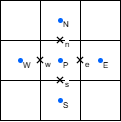
\includegraphics[width=0.25\linewidth]{Media/MeshDiagram.png}
    \caption{Node distribution for a single control volume $P$. Subindexes for each adjacent node correspond to their cardinal direction relative to the main node. Using the capitalized letter to represent values located at the adjacent node centroid ($W$, $E$, $S$, $N$) and the uncapitalized alternative for values located at the wall corresponding to the interaction between the main node and the adjacent node.}
    \label{figMeshDiagram}
\end{figure}


\subsection*{Governing Transport Equations}
When studying transport phenomena, there are two main mechanisms that govern the propagation of a transport variable $\phi$. These are known as \textbf{Convection} and \textbf{Diffusion}, and classify the phenomena depending on what causes the transport of the transport variable $\phi$. Diffusion refers to transport caused by molecular movement within the body, while Convection refers to transport caused by bulk movement of the body. The governing transport equation for this phenomena is given by Eq.~\eqref{eqTransGov}, which is separated into four terms relating to the physical variation of $\phi$. The accumulation term describes the magnitude variation over time, the convective term describes the variation due to convection, the diffusive term describes the variation due to diffusion, and the source term describes any additional source contributions.

\begin{equation} \label{eqTransGov}
    \overbrace{\frac{\partial (\rho \phi)}{\partial t}}^{\text{Accumulation}} + \overbrace{\nabla (\rho v \phi)}^{\text{Convective}} = \overbrace{\nabla (\Gamma \nabla \phi)}^{\text{Diffusive}} + \overbrace{S_{P}}^{\text{Source}}
\end{equation}

The continuous governing equation needs to be integrated over a control volume $V_P$ with a defined time-step $\Delta t$. By applying the Gauss divergence theorem shown in Eq.~\ref{eqGaussDivergence}, the convective and diffusive terms can be converted into surface integrals, which will evaluate the flow through the cell interface.

\begin{equation}~\label{eqGaussDivergence}
    \int_{V_P} \frac{\partial (\rho \phi)}{\partial t} \, dV = \oint_{\partial V_P} \rho \mathbf{v} \phi \cdot \hat{n} \, dA = \oint_{\partial V_P} \Gamma \nabla \phi \cdot \hat{n} \, dA + \int_{V_P} S_P \, dV
\end{equation}

Each surface integral can then be approximated as a discrete sum over the four cell faces (west, east, south, north). The resulting discretized forms are shown by Eqs.~\eqref{eqTransAcc}--\eqref{eqTransConv}

\begin{equation}~\label{eqTransAcc}
	\frac{\partial (\rho \phi)}{\partial t} = \rho \frac{\phi_P - \phi^0_P}{\Delta t}
\end{equation}

The accumulation term follows a first-order implicit approximation, where $\phi^0_P$ corresponds to the value of node $P$ at the current time-step and $\phi_P$ corresponds to the value at the next time-step.

\begin{equation}~\label{eqTransDiff}
    \oint_{\partial V_P} \Gamma \nabla \phi \cdot \hat{n} \, dA = \Gamma_w \frac{\phi_W - \phi_P}{d_{PW}} S_w - \Gamma_e \frac{\phi_P - \phi_E}{d_{PE}} S_e + \Gamma_s \frac{\phi_S - \phi_P}{d_{PS}} S_s - \Gamma_n \frac{\phi_P - \phi_N}{d_{PN}} S_n
\end{equation}

The diffusive term approximates the gradient at the face by interpolating the values from the adjacent nodes, multiplied by the diffusivity coefficient $\Gamma$ and the surface at the interface $S_k$, and dividing by the distance between the central node and one of the adjacent nodes $d_{PK}$.

\begin{equation}~\label{eqTransConv}
    \oint_{\partial V_P} \rho \mathbf{v} \phi \cdot \hat{n} \, dA = \rho (v_e \phi_E S_e - v_w \phi_W S_w + v_n \phi_N S_n - v_s \phi_S S_s)
\end{equation}

The convective term uses the velocity components located at the cell wall faces, considered in the expression with their corresponding geometrical surface value. For this term, the convective scheme can considerably change the behaviour of the model.

By substituting all previously mentioned equations and organizing the different terms, the expression can be reorganized to depend only on the magnitude of the current node $P$ and its neighbours. Eq.~\eqref{eqTransDisc} shows the standard FVM form for an interior cell with 4 adjacent nodes.

\begin{equation}~\label{eqTransDisc}
    a_P \phi_P = a_W \phi_W + a_E \phi_E + a_S \phi_S + a_N \phi_N + b_P
\end{equation}

The coefficients $a_W, a_E, a_S, a_N$ include the effect of both the diffusive and convective phenomena. When using this discretization, the coefficient for the current cell $a_P = a_W + a_E + a_S + a_N + a^0_P$ will respect diagonal dominance due to the presence of the accumulation term $a^0_P = \rho V_P / \Delta t$. This equation will be iteratively solved for every node in the discretized domain at each time-step. Each chapter will include a brief explanation of the specific expressions used for each coefficient for their respective application. 


\subsection*{Motivation}


\subsection*{Objectives}
\begin{enumerate}
    \item{Develope a modular FVM solver using C++ capable of accurately simulating transport phenomena of increasing complexity. Using several benchmark cases to validate the accuracy of the implementation at each stage of the model, and testing the performance and behaviour of the different numerical methods implemented in the model once validated.}
    \item{Expand the knowledge about numerical methods applied to CFD \& HT and use it to solve and understand the resolution methodology of complex transport phenomena. Simultaneously using the opportunity to further develope a consistent and organized code structure and learning more about C++ and its capabilities as a programming language.}
\end{enumerate}


\subsection*{Scope}
The model developed in this project will solve three main models, testing a variety of benchmark problems for each one of them.

\begin{enumerate}
    \item The \textbf{pure diffusion} model will evaluate a purely diffusive heat conduction test scenario in 1D and 2D. This first model has the simplest discretization and will serve as a base implementation to test the data structure design for the code implementation. It will also serve as a first introduction to numerical parameters such as the time-step and temporal scheme, and allow for testing to be done regarding their effect on the performance of the model. For the 1D case, the code will be validated against the analytical solution for all implemented boundary combinations in a \textbf{1D Rod Case}. For the 2D case, the model will be validated against the \textbf{4 Materials Case} benchmark published by PENDING REFERENCE~\cite{}. In addition, this first case will be used to compare the Gauss-Seidel (GS) and Conjugate Gradient (CG) numerical algorithms in terms of performance.
    \item The \textbf{convection-diffusion} model will evaluate a complete convection-diffusion in 2D showing the spatial evolution of a transport variable for a fixed flow field. This model completes the transport equation and also introduces the discretization model proposed by Patankar~\cite{Patankar}, which implements a multi-scheme model for the convective scheme. The model will be validated against the \textbf{Smith-Hutton Case} benchmark published by PENDING REFERENCE~\cite{}. This section will also require the implementation of a new BiConjugate Gradient Stabilized (BiCGSTAB) numerical solver algorithm to solve the complexities introduced by the convective term.
    \item The \textbf{Navier-Stokes} model will evaluate a coupled 2D Navier-Stokes solver. This model will introduce the concepts of Fractional Step Method (FSM) and Staggered Meshes, requiring a severe overhaul for the code structure. The NS equation model can be simplified in multiple ways, depending on the physical phenomena trying to be described. As such, two different test scenarios of increasing complexity will be evaluated. The first one consists of the \textbf{Lid Driven Cavity Case} benchmark published by PENDING REFERENCE~\cite{}, which simplifies the model to include only the mass conservation component and the 2 momentum conservation components. The second case consists of the \textbf{Differentially Heated Cavity Case} benchmark published by PENDING REFERENCE~\cite{}, which introduces an additional energy conservation component. Fractional Step Method (FSM) and Staggered Meshes will also be introduced and their effect in model convergence will be studied.
\end{enumerate}


\section{Pure Diffusion Solver}~\label{chapDiffusion}
This chapter will explain the implementation of a pure diffusion model~\cite{FernandezOro, Versteeg2007}, which is the simplest version of a transport equation introduced in Chapter~\ref{chapIntroduction}. This scenario is obtained by setting the velocity field to zero ($\mathbf{v} = 0$), which eliminates the convective term from the expression. This case describes the physical phenomena of heat conduction through solid bodies, where energy is transmitted exclusively through diffusion as described by Fourier's Law, shown in Eq.~\eqref{eqFourier}. The simplicity of the model lends itself to be a good introduction for studying the numerical discretization and validating the core infrastructure of the code implementation. The core components \textbf{Material}, \textbf{Mesh}, \textbf{Discretizer}, \textbf{Solver}, and \textbf{Probe} were defined on this stage and will remain as the fundamental structure of the model moving forward.

\begin{equation}~\label{eqFourier}
    q_{cond} = - \lambda \nabla T
\end{equation}

Following the previously mentioned assumption of a stationary flow field, the convective term can be removed from the governing transport equation, reducing it to the expression shown in Eq.~\ref{eqDiffGov}. For a heat conduction phenomena, the diffusivity $\Gamma$ corresponds to the thermal conduction coefficient $\lambda$, while the source term $S_P$ corresponds to the internal heat generation $q_V$. As such, the expanded transport equation becomes Fourier's heat equation, shown in Eq.~\eqref{eqDiffGov}.

\begin{equation}~\label{eqDiffGov}
        \rho c_P\frac{\partial T}{\partial t} = \nabla (\lambda \nabla T) + q_{V}
\end{equation}

Integrating Eq.~\eqref{eqDiffGov} over the control volume $V_P$ and a time step $\Delta t$, and applying the Gauss divergence theorem to convert the diffusion term from a volume integral into a surface integral across the cell faces, gives:

\begin{equation}~\label{eqDiffInt}
    \rho c_P V_P \frac{T_P - T^0_P}{\Delta t} =
    \oint_{\partial V_P} \lambda \nabla T \cdot \hat{n} \, dA + q_V V_P
\end{equation}

The surface integral is approximated as a discrete sum over the four cell faces. The face-normal gradient at each interface is evaluated by a central difference between the adjacent cell centroids, and the face conductivity $\lambda_k$ is computed from the harmonic mean of the adjacent cell values (Eq.~\eqref{eqHarmonicMean}):

\begin{equation}~\label{eqDiffFaceSum}
    \oint_{\partial V_P} \lambda \nabla T \cdot \hat{n} \, dA \approx
      \lambda_w S_w \frac{T_W - T_P}{d_{PW}}
    + \lambda_e S_e \frac{T_E - T_P}{d_{PE}}
    + \lambda_s S_s \frac{T_S - T_P}{d_{PS}}
    + \lambda_n S_n \frac{T_N - T_P}{d_{PN}}
\end{equation}

Substituting Eq.~\eqref{eqDiffFaceSum} into Eq.~\eqref{eqDiffInt} yields the fully discretized equation for node $P$:

\begin{equation}~\label{eqDiffDisc}
	\rho c_P V_P \frac{T_P - T^0_P}{\Delta t} = \lambda_w S_w \frac{T_W - T_P}{d_{PW}} + \lambda_e S_e \frac{T_E - T_P}{d_{PE}} + \lambda_s S_s \frac{T_S - T_P}{d_{PS}} + \lambda_n S_n \frac{T_N - T_P}{d_{PN}} + q_V V_P
\end{equation}

An important consideration for pure-diffusion problems is the evaluation of the face diffusivity $\Gamma_k$ when a cell face lies at a material interface. A simple arithmetic mean would overestimate the conductance between two dissimilar materials; the correct choice is the harmonic mean, which is consistent with the series-resistance analogy for heat conduction:

\begin{equation}~\label{eqHarmonicMean}
    \Gamma_k = \frac{2 \Gamma_P \Gamma_K}{\Gamma_P + \Gamma_K}
\end{equation}

For the thermal conduction model of this chapter, $\Gamma \equiv \lambda$.

By expanding Eq.~\eqref{eqDiffDisc} and reorganizing the terms the same expression shown in Eq.~\eqref{eqTransDisc} can be obtained for this particular problem. Table~\ref{tabDiffCoeff} shows a summary of the discretized coefficient expressions

\begin{table}
    \centering
    \begin{tabular}{|c|c|}
        \hline
        Coefficient & Expression \\
        \hline
        $a_W$ & $\dfrac{\lambda_w S_w}{d_{PW}}$ \\
        $a_E$ & $\dfrac{\lambda_e S_e}{d_{PE}}$ \\
        $a_S$ & $\dfrac{\lambda_s S_s}{d_{PS}}$ \\
        $a_N$ & $\dfrac{\lambda_n S_n}{d_{PN}}$ \\
        $b_P$ & $a^0_P T^0_P + q_V V_P$ \\
        \hline
    \end{tabular}
    \caption{Summary of discretized coefficients for standard FVM formulation for an interior cell. Where $a_k$ corresponds to the coefficient describing the interaction with an adjacent node, and $b_P$ is the right-hand side (RHS) term that describes the influence of the previous step and the source.}
    \label{tabDiffCoeff}
\end{table}

\subsection{Boundary Conditions}
Since boundary conditions are imposed instead of corresponding to the interaction of the center node with a neighboring node, their implementation in the code needs a special formulation. The current model supports 3 different types of boundary conditions; namely \textbf{Dirichlet}, \textbf{Neumann}, and \textbf{Robin}. The explanation concerning the implementation of boundary conditions will be done taking a west boundary as reference; the same concept detailed in this scenario will apply for the other boundaries with their respective coefficients. 

Dirichlet boundary conditions directly assign the variable value at the boundary. As such, the gradient can be approximated by using the distance between the cell centroid and the boundary wall $d_{Pw}$ and following the same discretization definitions shown in Table~\ref{tabDiffCoeff}. The coefficient term will be added to the diagonal coefficient $a_P$ and the assigned temperature is imposed by introducing it as part of $b_P$. 

\begin{equation}~\label{eqDiffBCDir}
    a_W = 0 \qquad
    a_P \mathrel{+}= D_w = \dfrac{\lambda_w S_w}{d_Pw} \qquad
    b_P \mathrel{+}= D_w T_{BC} \qquad
\end{equation}

Neumann boundary conditions assign the flux at the surface rather than the magnitude. As such, the flux value is already known at the surface and can be directly included into the RHS term of the discretization. No additional terms need to be added to the diagonal coefficient.

\begin{equation}~\label{eqDiffBCNeu}
    a_W = 0 \qquad
    b_P \mathrel{+}= q_{BC} S_w \qquad
\end{equation}

Robin boundary conditions, also known as convection / hybrid boundary conditions, impose a variable heat flux that relates the temperature at the node $T_P$ with the temperature of a far-away fluid $T_\infty$ through a convective heat transfer coefficient $h$. The resulting conductance term is added to the diagonal coefficient $a_P$ and to the RHS of the discretized equation.

\begin{equation}~\label{eqDiffBCRob}
    a_W = 0 \qquad
    a_P \mathrel{+}= h S_w \qquad
    b_P \mathrel{+}= h S_w T_\infty \qquad
\end{equation}

Implementation and validation of the 1D and 2D cases are discussed in the following subsections.

% Sections
\subsection{1D Transient Conduction - 1D Rod Case}~\label{secDiffusion1D}
In this section, the implementation of the heat conduction model for the \textbf{1D Rod Case} will be developed. The problem consists of a thin $1 m$  bar with adiabatic walls on the south/north faces and Dirichlet boundary conditions for the west/east faces. The west wall is set at $T_w = 100 ^\circ C$, while the eastern wall is set at $T_e = 20 ^\circ C$, with initial conditions set at $T_0 = 30 ^\circ C$. Furthermore, the rod is defined as being made of copper with properties $\lambda = 400 W/(m \cdot K)$, $\rho = 8960 kg/m^3$, and $c_P = 380 J/(kg \cdot K)$. A schematic of the problem is shown in Figure~\ref{fig1DRod}.

\begin{figure}[ht]
    \centering
    \includegraphics[width=0.45\linewidth]{Chapter1/Media/PLACEHOLDER.png}
    \caption{Diagram of 1D Rod Case, including original boundary conditions proposed for that case~\cite{}.}
    \label{fig1DRod}
\end{figure}


\subsubsection{Model Implementation}
The model implementation was designed to work using a configuration file that includes all the relevant parameters required to define a simulation. This ensures that the model will be robust enough to handle a wide range of simulations without needing any modifications. A summary of all the different parameters included in the file is shown in Table~\ref{tabDiffConfig1D}. A detailed explanation of each one of the groups and their relevant information is shown below. \textbf{Physical} includes the initial temperature and a list of the available materials and their thermophysical properties. \textbf{Geometrical} includes the geometric parameters; the model can only support rectangular shapes in this implementation and changes will be made when more complex geometries are studied. Sections must be defined with a material, the number of nodes for that specific section $N_s$, beginning and ending coordinates $x_0$ and $x_1$, and internal heat generation $q_V$. \textbf{Numerical} includes the numerical parameters; the model currently has both the Gauss-Seidel (GS) and Conjugate Gradient (CG) solvers implemented and both will be compared as a first step before performing the relevant studies discussed ahead. \textbf{Mesh} includes the option to choose from four different algorithms, as well as all relevant parameters for each of these alternatives. \textbf{Boundary Conditions} includes an array describing the boundaries for the model and can currently support Dirichlet, Neumann, and Convection boundary conditions. In addition, it supports variable temperatures for Dirichlet boundary conditions.

\begin{table}[ht]
	\centering
	\begin{tabular}{|l|c|p{0.5\linewidth}|}
		\hline
		Group & Parameter & Description \\
		\hline
		\multirow{3}{*}{Physical Data} & T0 & Initial value for temperature map. \\
					       & \multirow{2}{*}{materials} & List of vectors with thermophysical properties corresponding to each material. \\
		\hline
		\multirow{5}{*}{Geometrical Data} & width & Geometric dimension. \\
					          & height & Geometric dimension. \\
                              & \multirow{3}{*}{sections} & List of vectors indicating the distribution of materials in the simulation. Also includes amount of nodes and internal heat generation. \\
		\hline
		\multirow{7}{*}{Numerical Data} & scheme & Scheme for simulation. \\
					     & solver & Solver algorithm for simulation. \\
					     & maxIterations & Limit of iterations per timestep. \\
					     & endTime & Last instant of the simulation. \\
					     & timeStep & Time increment after each instant. \\
					     & tolNumeric & Tolerance for numerical solver. \\
					     & tolTemporal & Tolerance for steady-state convergence. \\
		\hline
		\multirow{5}{*}{Mesh Data} & meshAlgorithm & Algorithm for mesh generation. \\
					   & strength & Cubic algebraic mesh parameter. \\
					   & centering & Cubic algebraic mesh parameter. \\
					   & kappa & Power law mesh parameter. \\
					   & delta & Hyperbolic tangent mesh parameter. \\
		\hline
		\multirow{2}{*}{Boundary Data} & \multirow{2}{*}{boundaries} & List of vectors describing the boundary conditions on each side. \\
		\hline
	\end{tabular}
	\caption{Configuration file structure for 1D Rod Case. Showing the design structure for the metadata used to define the simulations.}
	\label{tabDiffConfig1D}
\end{table}


\subsubsection{Temporal Scheme}
One of the first numerical parameters to be evaluated in this project is the temporal scheme. This parameter determines the relevance that each time-step will have in the calculation of the next one. The \textbf{explicit} scheme, relies exclusively on information available from the current time-step, described as a function $f(T^{n-1})$ and requires a small enough time-step to ensure stability, given by Eq.~\eqref{eqDifftExplicit1D}. On the other hand, the \textbf{implicit} scheme relies exclusively on information from the time-step being currently calculated, being a function of $f(T^n)$. Finally, the \textbf{Crank-Nicolson} scheme employs a second-order scheme that averages the estimation made by both the explicit and implicit temporal schemes, being a function of $f(0.5 (T^{n-1} + T^n))$. 

\begin{equation}~\label{eqDifftExplicit1D}
    \Delta t_{max} = \frac{\Delta x^2}{2 \alpha}
\end{equation}


\subsubsection{Solver Comparison}
An additional decision to make when solving this kind of problems is the numerical solver to be used during simulations. While the matrix definition remains constant in both cases, as both require a sparse matrix in the form $A \mathbf{T} = b$, selecting the right solver can have a big impact in the performance of the solver. In this project, an initial comparison between the Gauss-Seidel (GS) and Conjugate Gradient (CG) algorithms will be made with the objective of evaluating performance and efficiency. A brief introduction to both algorithms is shown below before showing the results of said comparison.


\paragraph{Gauss-Seidel}
The GS method solves linear systems by iteratively cycling through each node in sequence and updating them by using the most recent values from its adjacent nodes. Each cell needs to be calculated directly by using Eq.~\eqref{eqSolverGS}, which delays the propagation of information from one cell to the others. While convergence is a guarantee when the matrix is diagonally dominant, it is susceptible to mesh size as it will directly impact the number of operations.

\begin{equation}~\label{eqSolverGS}
    T^{n+1}_P = \frac{1}{a_P} \left( b_P - \sum_{k \neq P} a_k T^*_{k} \right)
\end{equation}

\begin{algorithm}[ht]
\caption{Gauss-Seidel iterative solver}
\label{algGS}
\begin{algorithmic}[1]
    \Require Coefficient matrix $A$, RHS vector $\mathbf{b}$, initial guess $\mathbf{T}^0$, tolerance $\varepsilon$, maximum iterations $k_{\max}$
    \Ensure Solution vector $\mathbf{T}$
    \State $\mathbf{T} \gets \mathbf{T}^0$
    \For{$k = 1$ \textbf{to} $k_{\max}$}
        \For{$i = 1$ \textbf{to} $N$}
            \State $T_i \gets \dfrac{1}{a_{ii}} \!\left( b_i - \displaystyle\sum_{j \neq i} a_{ij}\, T_j \right)$
        \EndFor
        \If{$\|\mathbf{b} - A\mathbf{T}\| < \varepsilon$}
            \State \textbf{break}
        \EndIf
    \EndFor
    \Return $\mathbf{T}$
\end{algorithmic}
\end{algorithm}


\paragraph{Conjugate Gradient}
The CG method is an iterative Krylov subspace solver designed specifically for Symmetric Positive Definite (SPD) systems. For heat conduction problems, this matches the diffusion coefficient matrix since the interaction between two adjacent nodes is identical in both directions (symmetrical) and is diagonally dominant due to the accumulation term in $a_P$ (positive definite). Contrary to the GS method, rather than updating the values one by one, CG minimizes the residual over the sequence of search directions $\mathbf{p}_k$ that are mutually $A$-conjugate:

\begin{equation}~\label{eqSolverCG}
    \mathbf{p}^T_i A \mathbf{p}_j = 0, \qquad i \neq j
\end{equation}

This guarantees that no iteration undoes the progress made by previous ones. Because of this capacity of propagating information, CG converges in maximum $N$ iterations, being $N$ the amount of unknowns. It is also important to highlight that CG is only valid for SPD systems. As it will be explained in Chapter~\ref{chapConvection}, once symmetry is broken due to the convective term, the solver algorithm needs to be changed to a more generalized variant to be able to handle non-SPD scenarios.

\begin{algorithm}[ht]
\caption{Conjugate Gradient solver}
\label{algCG}
\begin{algorithmic}[1]
    \Require SPD coefficient matrix $A$, RHS vector $\mathbf{b}$, initial guess $\mathbf{T}^0$, tolerance $\varepsilon$, maximum iterations $k_{\max}$
    \Ensure Solution vector $\mathbf{T}$
    \State $\mathbf{r}^0 \gets \mathbf{b} - A\mathbf{T}^0$;\quad $\mathbf{p}^0 \gets \mathbf{r}^0$;\quad $\mathbf{T} \gets \mathbf{T}^0$
    \For{$k = 0, 1, 2, \ldots, k_{\max}$}
        \State $\alpha_k \gets \dfrac{\mathbf{r}^k \cdot \mathbf{r}^k}{\mathbf{p}^k \cdot A\,\mathbf{p}^k}$
        \State $\mathbf{T}^{k+1} \gets \mathbf{T}^k + \alpha_k\,\mathbf{p}^k$
        \State $\mathbf{r}^{k+1} \gets \mathbf{r}^k - \alpha_k\, A\,\mathbf{p}^k$
        \If{$\|\mathbf{r}^{k+1}\| < \varepsilon$}
            \State \textbf{break}
        \EndIf
        \State $\beta_k \gets \dfrac{\mathbf{r}^{k+1} \cdot \mathbf{r}^{k+1}}{\mathbf{r}^k \cdot \mathbf{r}^k}$
        \State $\mathbf{p}^{k+1} \gets \mathbf{r}^{k+1} + \beta_k\,\mathbf{p}^k$
    \EndFor
    \Return $\mathbf{T}^{k+1}$
\end{algorithmic}
\end{algorithm}


\paragraph{Results}
Solver performance is evaluated using two metrics: the number of inner iterations required to reach convergence at each time-step, and the final residual $\|\mathbf{b} - A\mathbf{T}\|$ after convergence. The comparison is carried out on the \textbf{1D Rod Case}~\cite{} extended with an internal heat source $q_V$, which introduces a parabolic steady-state profile that can be directly compared against the analytical solution given by Eq.~\eqref{eq1DAnalyticalSol}. Both solvers use $N = 100$ nodes, $\Delta t = 0.5\,\text{s}$, a Crank-Nicolson temporal scheme, and a uniform mesh. The results are shown in Figure~\ref{figDiffCompSolver}.

CG outperforms GS by a considerable margin on both metrics. This is consistent with the structural properties described above: the diffusion matrix is SPD, so CG propagates information globally through its $A$-conjugate search directions and is guaranteed to converge in at most $N$ steps. GS updates nodes one at a time, propagating information only one cell per iteration, and therefore requires many more sweeps to resolve long-range temperature gradients. Based on these results, CG was selected as the solver for all subsequent numerical studies in this chapter.

\begin{figure}[ht]
    \begin{tabular}{cc}
        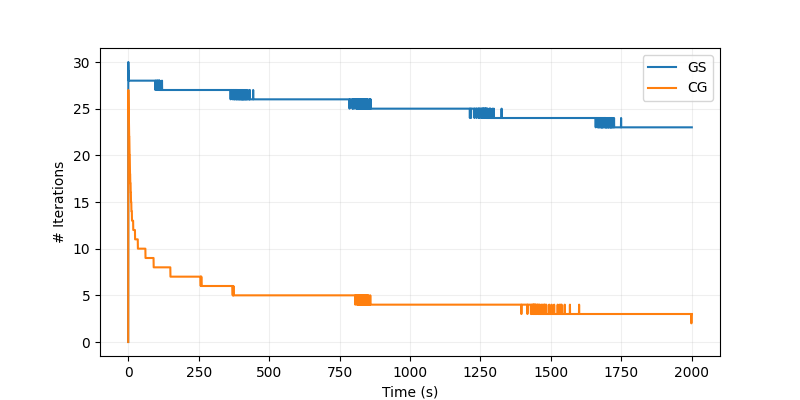
\includegraphics[width=0.45\linewidth]{Chapter1/Media/SolverComparisonIterations.png} & 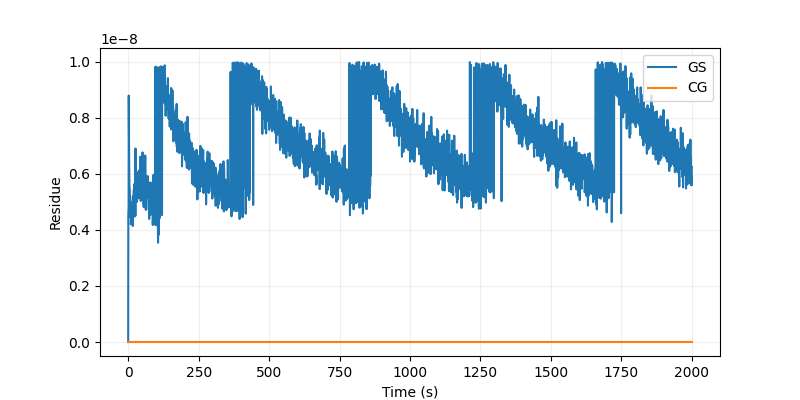
\includegraphics[width=0.45\linewidth]{Chapter1/Media/SolverComparisonResidue.png} \\
        \textit{Iterations} & \textit{Residue} \\
    \end{tabular}
    \caption{\textit{Performance comparison between Gauss-Seidel and Conjugate Gradient solvers. Number of iterations until solution (left) and solver residual after convergence (right).}}
    \label{figDiffCompSolver}
\end{figure}


\subsubsection{Numerical Parameters Study}
For this test, the time step $\Delta t$ and the number of nodes $N$ are modified to analyze the number of iterations and compare them with the analytical solution. Both parameters will be independently swept across their respective range of values, while keeping the other parameter at a constant value. A summary of the values for each one of these parameters is shown in Table \ref{tabDiffNumerical1D}, highlighting the values used for the base case.

\begin{table}[ht]
    \centering
    \begin{tabular}{|c|c|}
        \hline
        Parameter & Values \\
        \hline
        $\Delta t$ & 0.1, \textbf{0.5}, 1.0, 2.0, 5.0 \\
        $N$ & 50, \textbf{100}, 200, 400 \\
        \hline
    \end{tabular}
    \caption{\textit{Detail of numerical parameters to be studied. Each variable will remain at their respective highlighted value while the other one sweeps through their range.}}
    \label{tabDiffNumerical1D}
\end{table}


\paragraph{$\Delta t$ Sweep}
The results obtained from the tests explained above are shown in Figure \ref{figDiffResults1DA}. As expected, the number of iterations remains unchanged for the explicit scheme, as it is meant to be a direct calculation. On the other hand, both the Crank-Nicolson and implicit schemes require more iterations per time step as it increases. This is mainly due to the accumulation term decreasing in magnitude as $\Delta t$ increases, while the adjacent node coefficients do not decrease with $\Delta t$. This in turn makes the system less diagonally dominant and slower to converge. Compared to the analytical solution, the explicit scheme shows a significant error for $0.1 < \Delta t$, while a small increase could be seen for the Crank-Nicolson and implicit schemes. As a second-order accurate method, Crank-Nicolson shows lower error compared to implicit, which is a first-order accurate method. Overall, the Crank-Nicolson scheme has shown better performance in terms of number of iterations needed and precision compared to the analytical solution. Furthermore, the results for explicit seem to stagnate at a constant value after the lowest time step value tested, suggesting that the limit set by Eq. \ref{eqDifftExplicit1D} has been exceeded. The computation time is seen to be similar between the Crank-Nicolson and implicit schemes, with a small advantage for the implicit scheme.

\begin{figure}[ht]
    \begin{tabular}{cc}
        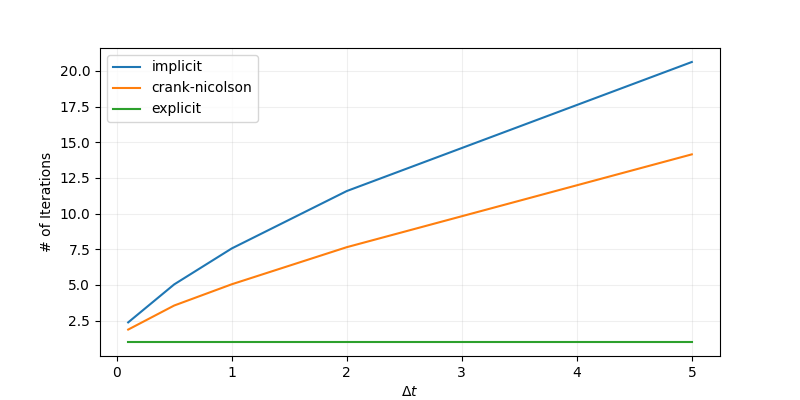
\includegraphics[width=0.45\linewidth]{Chapter1/Media/tSweepIterations.png} & 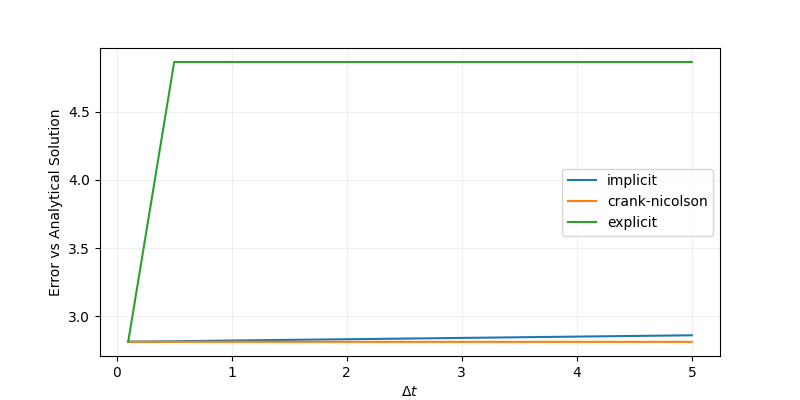
\includegraphics[width=0.45\linewidth]{Chapter1/Media/tSweepAnalytical.png} \\
        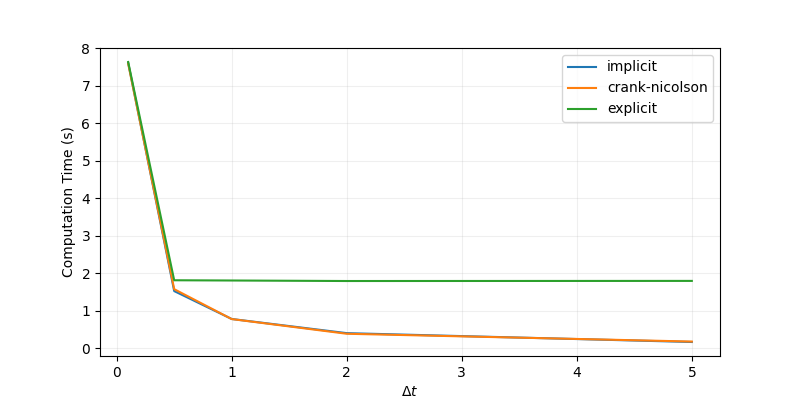
\includegraphics[width=0.45\linewidth]{Chapter1/Media/tSweepTime.png} & 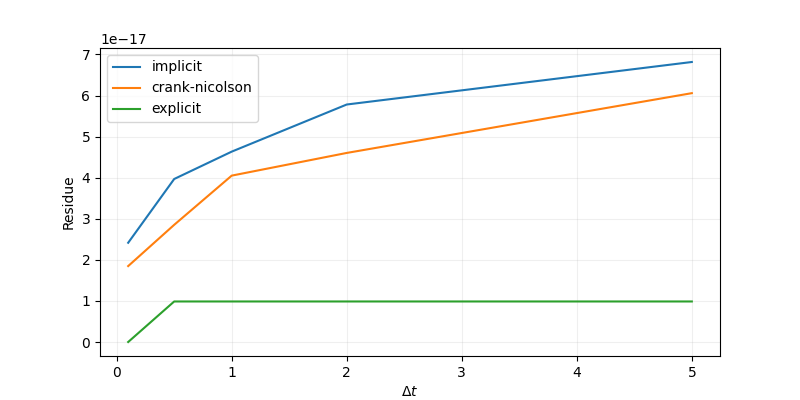
\includegraphics[width=0.45\linewidth]{Chapter1/Media/tSweepResidue.png} \\
    \end{tabular}
    \caption{\textit{$\Delta t$ sweep results.}}
    \label{figDiffResults1DA}
\end{figure}


\paragraph{$N$ Sweep}
The results obtained for the tests explained above are shown in Figure \ref{figDiffResults1DB}. Similarly to the previous case, the explicit scheme is a direct calculation and does not require more iterations. In addition, both the Crank-Nicolson and implicit schemes show an increase in the number of iterations as the mesh is refined, with Crank-Nicolson showing better performance overall. Since a larger mesh means more finite volumes, the amount of calculations performed by the model will increase. Compared to the analytical solution, the explicit scheme still showed higher values when compared to the Crank-Nicolson and implicit schemes; however, it seems to get closer as the number of nodes increases. In terms of computation time, both the Crank-Nicolson and implicit schemes saw a slight increase, while the explicit scheme saw a major difference as the mesh got finer.

\begin{figure}[ht]
    \begin{tabular}{cc}
        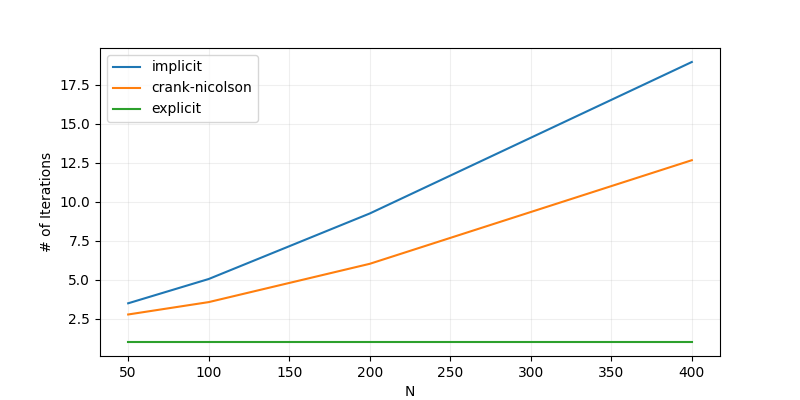
\includegraphics[width=0.45\linewidth]{Chapter1/Media/NSweepIterations.png} & 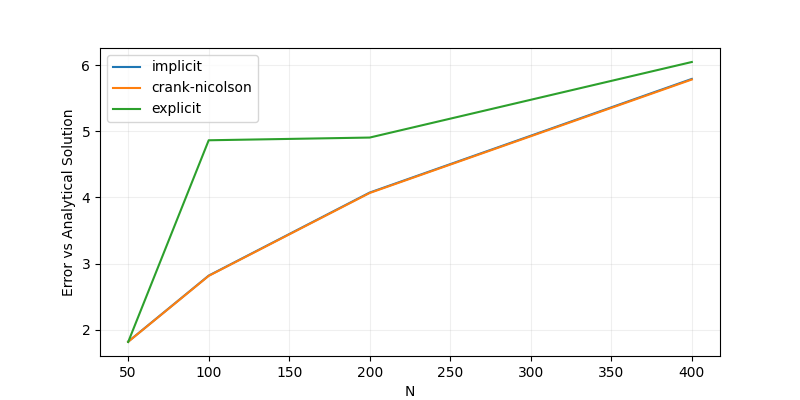
\includegraphics[width=0.45\linewidth]{Chapter1/Media/NSweepAnalytical.png} \\
        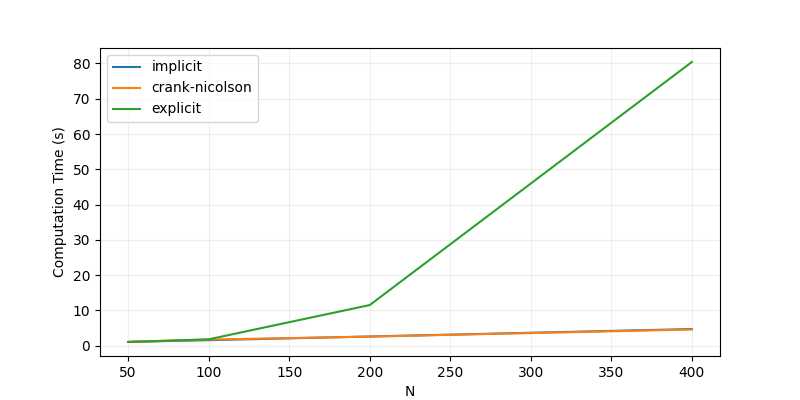
\includegraphics[width=0.45\linewidth]{Chapter1/Media/NSweepTime.png} & 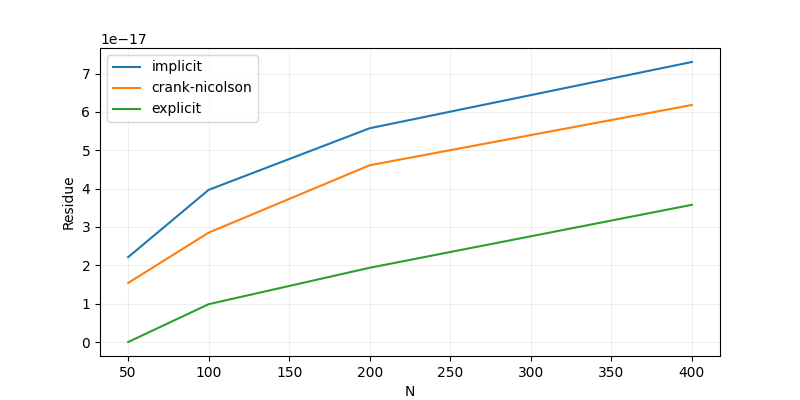
\includegraphics[width=0.45\linewidth]{Chapter1/Media/NSweepResidue.png} \\
    \end{tabular}
    \caption{\textit{$N$ sweep results.}}
    \label{figDiffResults1DB}
\end{figure}


\subsubsection{Model Validation}
In addition to the Dirichlet boundary condition established in the problem statement, Neumann and Convection boundary conditions have also been implemented in the model. Furthermore, support for variable temperatures for Dirichlet boundary conditions was implemented. To validate this implementation, a comparison will be made with the analytical solution for a steady-state scenario with the transient-state model once it reaches equilibrium.

At steady state the time derivative vanishes and the 1D governing equation reduces to:

\begin{equation}~\label{eq1DAnalytical}
    \frac{d}{dx}\!\left(\lambda \frac{dT}{dx}\right) + q_V = 0
\end{equation}

For uniform $\lambda$ and $q_V = 0$, this integrates to a linear temperature profile $T(x) = A + Bx$, with constants $A$ and $B$ determined by the two boundary conditions. Table~\ref{tabDiff1DAnalytical} summarises the closed-form solutions for each of the five boundary-condition pairs tested. For Cases 2 and 4 (Robin), the temperature at the convective wall $T^*$ follows from the continuity of heat flux between the fluid and the solid at steady state.

\begin{table}[ht]
    \centering
    \renewcommand{\arraystretch}{2.2}
    \begin{tabular}{|c|l|l|}
        \hline
        Case & Boundary Conditions & Analytical Solution $T(x)$ \\
        \hline
        1 & Neumann (W) -- Dirichlet (E)
          & $T_E + \dfrac{\dot{q}_W}{\lambda}(L - x)$ \\
        2 & Robin (W) -- Dirichlet (E)
          & $T_w^* + (T_E - T_w^*)\dfrac{x}{L}$,\quad $T_w^* = \dfrac{hL\,T_\infty + \lambda\,T_E}{hL + \lambda}$ \\
        3 & Dirichlet (W) -- Neumann (E)
          & $T_W + \dfrac{\dot{q}_E}{\lambda}\,x$ \\
        4 & Dirichlet (W) -- Robin (E)
          & $T_W + (T_e^* - T_W)\dfrac{x}{L}$,\quad $T_e^* = \dfrac{\lambda\,T_W + hL\,T_\infty}{\lambda + hL}$ \\
        5 & Variable Dirichlet (W) -- Dirichlet (E)
          & $T_W(t) + \bigl(T_E - T_W(t)\bigr)\dfrac{x}{L}$,\quad $T_W(t) = 100 + 50\cos\!\!\left(\dfrac{0.01\,t}{5\pi}\right)$ \\
        \hline
    \end{tabular}
    \caption{Analytical steady-state solutions for each boundary-condition pair. $\dot{q}_W$ and $\dot{q}_E$ denote the prescribed heat flux entering the domain at the west and east faces respectively; $h$ is the convective heat transfer coefficient and $T_\infty$ the far-field fluid temperature.}
    \label{tabDiff1DAnalytical}
\end{table}

A summary of the pairs of boundary conditions used for the tests is shown in Table~\ref{tabDiff1DBoundaryCases}, while comparisons with the steady-state solution are shown in Figure~\ref{figDiff1DAnalSol}. An additional case is included to test the proper implementation of the variable temperature Dirichlet boundary condition. As shown, all pairs evaluated accurately matched the analytical solution. Furthermore, the configuration file can now provide mathematical expressions instead of constant values when defining Dirichlet boundary conditions, as shown by the temperature profile in Case 5. This capability can now easily be scaled up towards other functions in the model.

\begin{table}[ht]
    \centering
    \begin{tabular}{|c|c|}
        \hline
        Case & Boundary Conditions \\
        \hline
        1 & Neumann-Dirichlet \\
        2 & Convection-Dirichlet \\
        3 & Dirichlet-Neumann \\
        4 & Dirichlet - Convection \\
        5 & $T_{(t)} = 100 + 50 \cos \left( \frac{0.01 t}{5 \pi} \right)$ \\
        \hline
    \end{tabular}
    \caption{\textit{Cases for model validation. Each case describes a Left-Right pair of boundary conditions to be tested with the 1D Rod Case.}}
    \label{tabDiff1DBoundaryCases}
\end{table}

\begin{figure}[ht]
    \begin{tabular}{cc}
        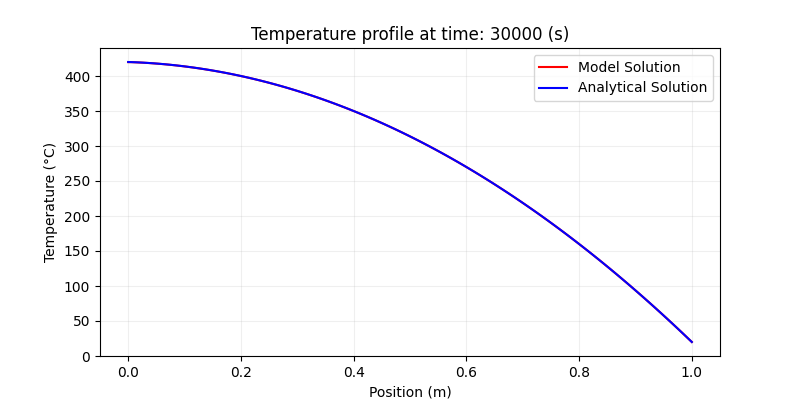
\includegraphics[width=0.45\linewidth]{Chapter1/Media/BoundaryND.png} & 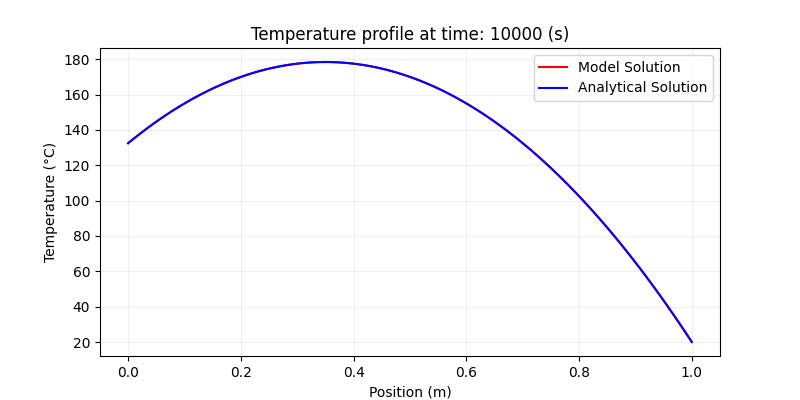
\includegraphics[width=0.45\linewidth]{Chapter1/Media/BoundaryCD.png} \\
	\scriptsize{\textit{Case 1}} & \scriptsize{\textit{Case 2}} \\
        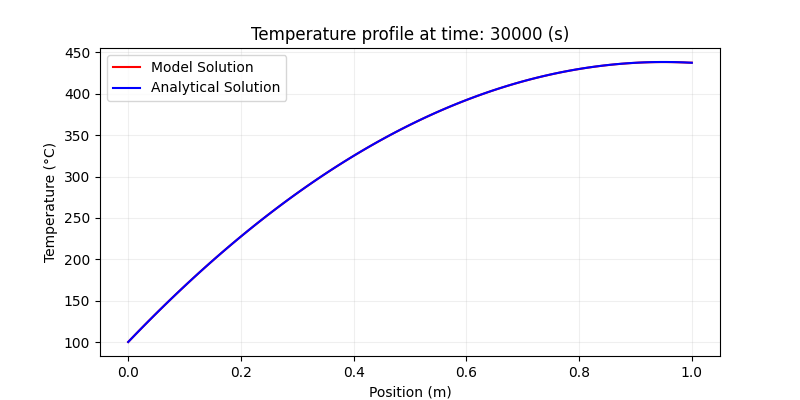
\includegraphics[width=0.45\linewidth]{Chapter1/Media/BoundaryDN.png} & 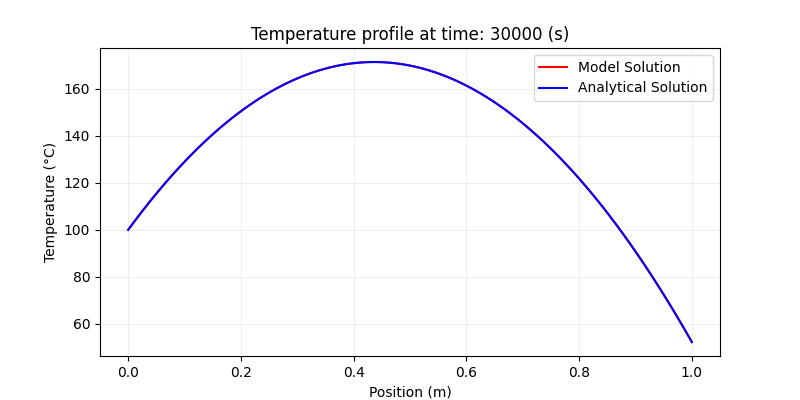
\includegraphics[width=0.45\linewidth]{Chapter1/Media/BoundaryDC.png} \\
	\scriptsize{\textit{Case 3}} & \scriptsize{\textit{Case 4}} \\
        \multicolumn{2}{c}{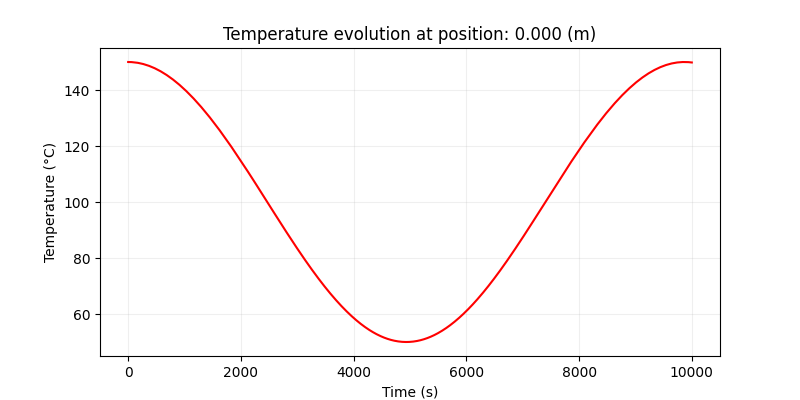
\includegraphics[width=0.45\linewidth]{Chapter1/Media/BoundaryVD.png}} \\
	\multicolumn{2}{c}{\scriptsize{\textit{Case 5}}} \\
    \end{tabular}
    \caption{\textit{Comparison of model results with analytical solutions and implementation of mathematical expression reading for Dirichlet boundary condition.}}
    \label{figDiff1DAnalSol}
\end{figure}


\subsection{2D Transient Conduction - 4 Materials Case}~\label{secDiffusion2D}
In this section, the implementation of a heat conduction model for the \textbf{4 Materials Case} will be developed. The problem consists of the rectangular domain shown in Fig.~\ref{fig4Materials}, which is composed by 4 different materials with their thermophysical properties being listed in Table~\ref{tab2DMaterials}. Furthermore, the domain has an initial value of $T_0 = 8 ^\circ C$ and is bound by the boundary conditions shown in Table~\ref{tab4MaterialBC}.

\begin{figure}[ht]
    \centering
    \includegraphics[width=0.45\linewidth]{Chapter1/Media/PLACEHOLDER.png}
    \caption{Diagram for 4 Materials Case.}
    \label{fig4Materials}
\end{figure}

\begin{table}[ht]
    \centering
    \begin{tabular}{|c|c|c|c|}
        \hline
        \multirow{2}{*}{Material} & $\rho$ & $c_P$ & $\lambda$ \\
                                  & $[kg/m^3]$ & $[J/(kg \cdot K)]$ & $[W/(mK)]$ \\
        \hline
        M1 & 1500 & 750 & 160 \\ 
        M2 & 1600 & 770 & 140 \\
        M3 & 1900 & 810 & 200 \\
        M4 & 2500 & 930 & 140 \\
        \hline
    \end{tabular}
    \caption{Thermophysical properties of the four materials in the domain.}
    \label{tab2DMaterials}
\end{table}

\begin{table}[ht]
    \centering
    \begin{tabular}{|c|l|}
        \hline
        Cavity Wall & Boundary Condition \\
        \hline
        West & \textbf{Robin}: In contact with fluid at $T_f = 33 ^\circ C$ and $h = 9 \, W/(m^2 K)$ \\
        East & \textbf{Dirichlet}: Uniform temperature $T(t) = 8 + 0.005 t ^\circ C$ \\
        South & \textbf{Dirichlet}: Uniform temperature $T = 23 ^\circ C$ \\
        North & \textbf{Neumann}: Uniform $\dot{Q}_{flow}$ \\
        \hline
    \end{tabular}
    \caption{Boundary conditions for the 4 Materials Case domain.}
    \label{tab4MaterialBC}
\end{table}


\subsubsection{Model Implementation}
The model developed for the 2D case will follow the same discretization proposed earlier for the 1D case. However, some modifications to the code structure were needed to support the new functionalities. For example, Probe was expanded to support different types of probes with a better control over the region of the domain that is desired. A summary of the modified parameters included in this iteration of the model is shown in Table~\ref{tabConfig2D}, summarizing the new parameters in the configuration file. As shown, Probes have now been added as a configurable parameter to allow the user to choose which data is being saved. In addition, refinement was modified to be defined independently for each axis and in separate regions to allow the user better control over the mesh. Furthermore, a Medic class was also included to handle diagnostics and validation of energy conservation in the system. This class is also used as the central tool for debugging as it can easily be modified to log any information relevant to the model.

\begin{table}[ht]
	\centering
	\begin{tabular}{|l|c|p{0.5\linewidth}|}
		\hline
		Group & Parameter & Description \\
		\hline
        \multirow{4}{*}{Mesh Data} & \multirow{2}{*}{N} & List specifying total number of nodes for each axis. \\
					   & \multirow{2}{*}{refinement} & List of vectors specifying refinement configuration for each axis. \\
		\hline
		\multirow{2}{*}{Probe Data} & \multirow{2}{*}{probes} & List of vectors specifying the probes configured for the simulation. \\
		\hline
	\end{tabular}
	\caption{Configuration file structure changes, highlighting the expansion in mesh refinement capacity and probe flexibility.}
	\label{tabConfig2D}
\end{table}

\subsubsection{Numerical Parameter Study}
For this test, timestep $\Delta t$ and number of nodes $N$ are modified to analyze their impact on the number of iterations and total residue. Both parameters will be independently swept across their respective range of values while keeping the other parameter at a constant value. A summary of the values for each of these parameters is shown in Table \ref{tabDiffNumerical2D}, highlighting the values used for the base case. In addition, the explicit scheme still requires an imposed limit for the value of $\Delta t$; however the expression for the 2D case changes as described by Eq. \ref{eqDiffExplicit2D} due to the presence of simultaneous diffusion in both axis. Contrary to the results shown for the 1D case, there will be no comparison of error with the analytical solution or computation time. This numerical parameter study will focus on comparing the number of iterations and total residue.

\begin{table}[ht]
	\centering
	\begin{tabular}{|c|c|}
		\hline
		Parameter & Values \\
		\hline
		$\Delta t$ & 0.1, 0.5, \textbf{1.0}, 2.0, 5.0 \\
		$N$ & 50, \textbf{100}, 200, 400 \\
		\hline
	\end{tabular}
	\caption{Value ranges for numerical parameter study.}
	\label{tabDiffNumerical2D}
\end{table}

\begin{equation}
	\label{eqDiffExplicit2D}
\Delta t_{max} = \frac{\Delta x^2 \Delta y^2}{2 \alpha (\Delta x^2 + \Delta y^2)}
\end{equation}

\paragraph{$\Delta t$ Study}
The results obtained from the tests explained above are shown in Figure \ref{figDiffResults2DA}. As shown, the number of iterations and total residue follow a similar trend to the one seen in the 1D case, increasing with $\Delta t$ for the implicit and Crank-Nicolson schemes, showing a better performance for the Crank-Nicolson scheme on both metrics.  On the other hand, the explicit scheme did not present any changes during the timestep study. This is due to the timestep being limited by the expression discussed above; which activated for all analyzed cases.

\begin{figure}[ht]
	\begin{tabular}{cc}
		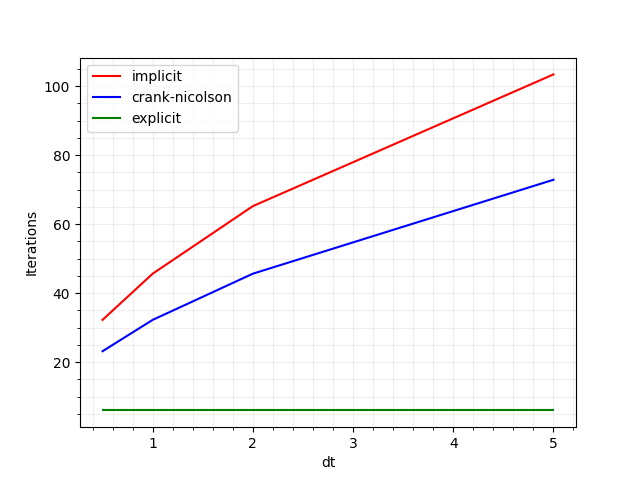
\includegraphics[width=0.45\linewidth]{Chapter1/Media/tSweep2DIterations.png} & 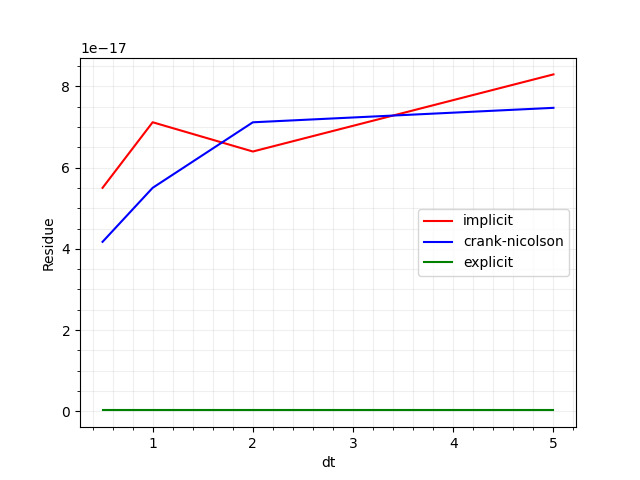
\includegraphics[width=0.45\linewidth]{Chapter1/Media/tSweep2DResidue.png} \\
	\end{tabular}
	\caption{$\Delta t$ sweep results.}
	\label{figDiffResults2DA}
\end{figure}

\paragraph{$N$ Study}
The results obtained from the tests explained above are shown in Figure \ref{figDiffResults2DB}. Just like in the previous test, the presented plots show a similar trend to the one seen in the previous scenario, showing an increase in number of iterations and residue for most cases. Furthermore, the implicit scheme showed higher sensitivity to increases in $N$ compared to the Crank-Nicolson and explicit schemes; with the explicit scheme showing no change at all. On the other hand, while residue was significantly higher for implicit on coarser meshes, the difference between the implicit and Crank-Nicolson schemes became smaller as $N$ increased; with the explicit scheme showing a slight increase in the beginning but less of an impact as $N$ kept increasing.

\begin{figure}[ht]
    \centering
	\begin{tabular}{cc}
		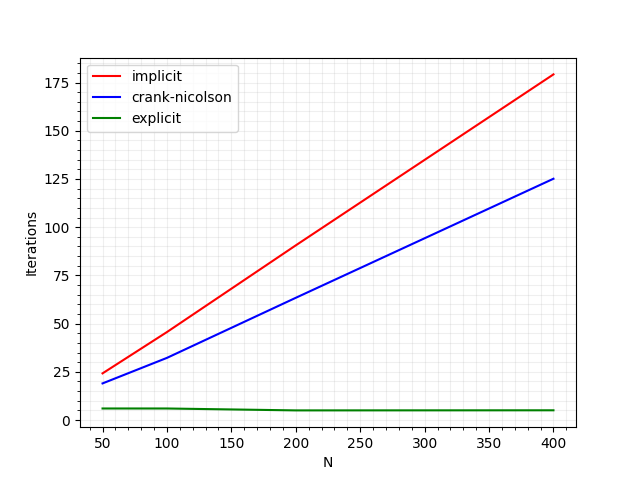
\includegraphics[width=0.45\linewidth]{Chapter1/Media/NSweep2DIterations.png} & 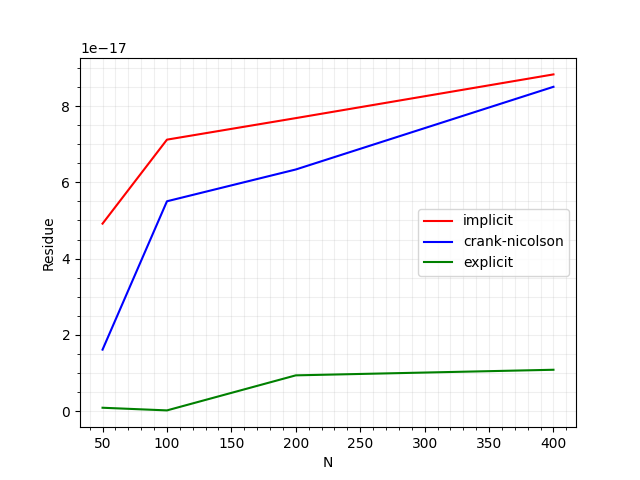
\includegraphics[width=0.45\linewidth]{Chapter1/Media/NSweep2DResidue.png} \\
	\end{tabular}
	\caption{$N$ sweep results.}
	\label{figDiffResults2DB}
\end{figure}

\subsubsection{Model Validation}
As a preliminary step, the three boundary condition types (Dirichlet, Neumann, and Robin) were independently verified in 2D by applying an adiabatic Neumann condition ($\partial T / \partial n = 0$) on the faces of the secondary axis, effectively reducing the problem to a 1D configuration along the primary axis. The results successfully replicated the steady-state profiles validated in Section~\ref{secDiffusion1D} for each axis, confirming that the boundary condition implementation is correct in two dimensions.

The primary benchmark for this chapter is the \textbf{4 Materials Case}~\cite{}, whose results are shown in Fig.~\ref{figDiff2D4Materials}. Since this is a transient simulation, no closed-form analytical solution exists; validation is instead performed against reference temperatures at two probe locations, $[0.65, 0.56]$ and $[0.74, 0.72]$, at prescribed time instants. The model successfully matched both reference values and produced a temperature distribution consistent with the expected evolution of the domain.

\begin{figure}[ht]
	\centering
	\begin{tabular}{cc}
		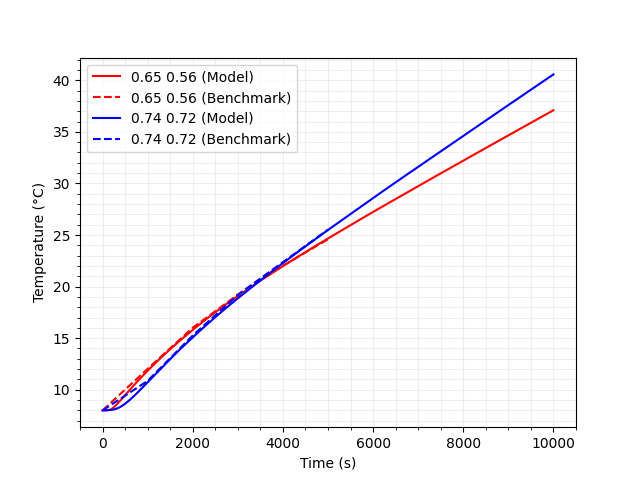
\includegraphics[width=0.45\linewidth]{Chapter1/Media/4MaterialsPoint.png} & 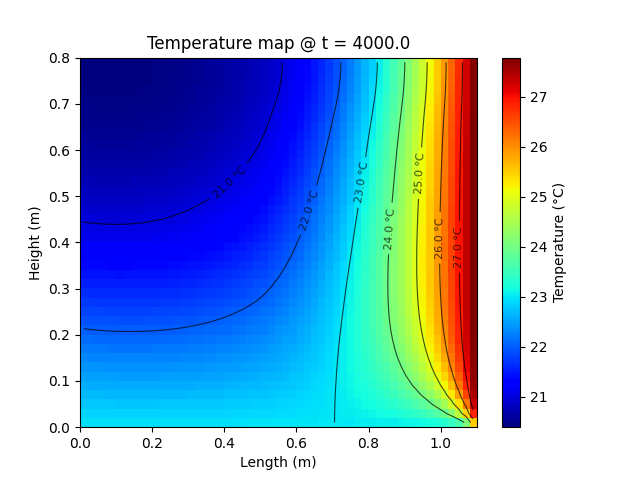
\includegraphics[width=0.45\linewidth]{Chapter1/Media/4MaterialsMap.png} \\
	\end{tabular}
	\caption{Comparison of probe temperatures against reference values (left) and steady-state temperature distribution (right) for the 4 Materials Case.}
	\label{figDiff2D4Materials}
\end{figure}



\section{Convection-Diffusion Model}~\label{chapConvection}

This chapter will explain the implementation of a convection-diffusion model. In this case, the complete transport equation shown in Chapter~\ref{chapIntroduction} needs to be implemented, considering both the diffusive and convective elements. The model implementation will be validated by solving the Smith-Hutton case and comparing the results to available reference values. In addition, the implementation described in this chapter will follow the discretization model described by Patankar~\cite{Patankar}, which proposes a generalized formulation that considers the various convective schemes available for numerical resolution. Based on said formulation, the discretized coefficients for a 2D model are shown below in Eqs.~\ref{eqConv_aw},~\ref{eqConv_ae},~\ref{eqConv_as},~\ref{eqConv_an},~\ref{eqConv_ap},~\ref{eqConv_bp}.

\begin{equation}~\label{eqConv_aw}
    a_W = D_w A(|P_w|) + ||F_w, 0||
\end{equation}

\begin{equation}~\label{eqConv_ae}
    a_E = D_e A(|P_e|) + ||-F_e, 0||
\end{equation}

\begin{equation}~\label{eqConv_as}
    a_S = D_s A(|P_s|) + ||F_s, 0||
\end{equation}

\begin{equation}~\label{eqConv_an}
    a_N = D_n A(|P_n|) + ||-F_n, 0||
\end{equation}

\begin{equation}~\label{eqConv_ap}
    a_P = a_W + a_E + a_S + a_N + a^0_P
\end{equation}

\begin{equation}~\label{eqConv_bp}
    b_P = S_{\phi} V_P + a^0_P \phi^0_P
\end{equation}

\begin{equation*}
    a^0_P = \frac{\rho^0_P V_P}{\Delta t}
\end{equation*}

As mentioned above, this discretization model includes the additional $A(|P|)$ term, which corresponds to a different function depending on the convective scheme. A summary of the expressions used for the convective schemes implemented in the model is shown in Table~\ref{tabConvSchemes}.

\begin{table}[ht]
    \centering
    \begin{tabular}{|c|c|}
        \hline
        Scheme & $A(|P|)$ \\
        \hline
        CDS & $1 - 0.5 |P|$ \\
        UDS & $1$ \\
        Hybrid & $\Vert 0, 1 - 0.5 |P| \Vert$ \\
        Power Law & $\Vert 0, (1 - 0.1|P|)^5 \Vert$ \\
        Exponential & $\frac{|P|}{e^{|P|} - 1}$ \\
        \hline
    \end{tabular}{}
    \caption{\textit{The function $A(|P|)$ for different schemes}~\cite{Patankar}.}
    \label{tabConvSchemes}
\end{table}

% Sections
\subsection{2D Convection-Diffusion - Smith-Hutton Case}~\label{secConvection2D}
The Smith-Hutton problem~\cite{SmithHutton1982} is a widely used benchmark for convection-diffusion schemes. It consists of a rectangular domain $[-1, 1] \times [0, 1]$ subject to a prescribed, analytically divergence-free velocity field:

\begin{equation}~\label{eqSHVelocity}
    u = 2y(1 - x^2), \qquad v = -2x(1 - y^2)
\end{equation}

This velocity field generates a circular flow that enters along the bottom from the left, sweeps across the domain, curves upward near the east boundary, and returns from right to left along the top. Because $\nabla \cdot \mathbf{v} = 0$ is satisfied analytically, the discrete continuity correction term in Eq.~\eqref{eqConv_ap} vanishes exactly, making this a clean test of the convective discretisation alone. A schematic of the problem is shown in Fig.~\ref{figSHDomain}.

\begin{figure}[ht]
    \centering
    \includegraphics[width=0.45\linewidth]{Chapter2/Media/PLACEHOLDER.png}
    \caption{Smith-Hutton problem domain and velocity streamlines~\cite{SmithHutton1982}.}
    \label{figSHDomain}
\end{figure}

The transport variable $\phi$ represents a passive scalar carried by the flow. Boundary conditions are:

\begin{itemize}
    \item \textbf{South inlet} ($y = 0,\ -1 \leq x \leq 0$): Dirichlet profile $\phi = 1 + \tanh\!\bigl(10(2x + 1)\bigr)$, which ramps from $0$ at $x = -1$ through $1$ at $x = -0.5$ to $2$ at $x = 0$.
    \item \textbf{South outlet} ($y = 0,\ 0 \leq x \leq 1$): Neumann zero-gradient $\partial \phi / \partial n = 0$.
    \item \textbf{All remaining walls}: Dirichlet $\phi = 0$.
\end{itemize}

The steep inlet profile makes this a demanding benchmark: a high-order scheme must resolve the sharp gradient without introducing oscillations, while an upwind scheme will smear it due to numerical diffusion. The problem is parameterised by the ratio $\rho/\Gamma$, which controls the global Peclet number. Three cases are tested: $\rho/\Gamma = 10^1$, $10^3$, and $10^6$, with $\Gamma = 1$ held fixed throughout. Validation is performed by comparing the computed exit profile $\phi(x,\, y=0)$ for $0 \leq x \leq 1$ against the reference values provided by Smith and Hutton~\cite{SmithHutton1982}.


\subsubsection{Model Implementation}
The convection-diffusion solver is built on the same modular architecture as Chapter~\ref{chapDiffusion}, extending it with three key additions. First, the velocity field is no longer a fixed parameter but a prescribed analytical input: the two components $u$ and $v$ are specified as mathematical expressions in the configuration file, which are parsed and evaluated at each cell face during the assembly of the convective fluxes $F_k$. This approach keeps the model general, allowing any analytically defined, divergence-free velocity field to be tested without modifying the source code. Second, ghost nodes are used at all domain boundaries (see Section~\ref{chapConvection}) instead of the half-cell wall treatment of Chapter~\ref{chapDiffusion}, enabling a consistent treatment of both the diffusive and convective face fluxes. Third, a new Boundary probe type was added to the Probe class, which records $\phi$ along a specified boundary face at each saved time-step; this is required for the Smith-Hutton validation, which compares the exit profile at the south outlet.

A summary of all configuration parameters for this model is shown in Table~\ref{tabConfigConv}. Compared to the previous chapter, the main additions are the \textbf{spatScheme} parameter for the convective scheme, the \textbf{velocityField} entry for the analytical velocity expressions, and the \textbf{medicOn} flag that activates the diagnostic tool.

\begin{table}[ht]
	\centering
	\begin{tabular}{|l|c|p{0.5\linewidth}|}
		\hline
		Group & Parameter & Description \\
		\hline
		\multirow{8}{*}{Numerical Data} & tempScheme & Temporal scheme selection for simulation. \\
            & spatScheme & Convective scheme selection for simulation. \\
            & solver & Solver algorithm for simulation. \\
			& tolNumeric & Tolerance for the numerical solver. \\
			& tolTemporal & Tolerance for the steady-state convergence. \\
			& maxIterations & Limit of iterations per time-step. \\
			& endTime & Last instant of the simulation. \\
			& timeStep & Time increment after each instant. \\
		\hline
		\multirow{4}{*}{Physical Data} & T0 & Initial value for $\phi$ over the domain. \\
					       & \multirow{2}{*}{materials} & List of vectors with thermophysical properties corresponding to each material. \\
                           & velocityField & Mathematical expressions for each velocity component. \\
		\hline
		\multirow{5}{*}{Geometrical Data} & width & Dimension of the domain in the secondary axis. \\
						  & \multirow{4}{*}{sections} & List of vectors indicating the material distribution. Also includes node count and internal source. \\
		\hline
		\multirow{9}{*}{Mesh Data} & strength & Cubic algebraic mesh parameter. \\
					   & centering & Cubic algebraic mesh parameter. \\
					   & kappa & Power law mesh parameter. \\
					   & delta & Hyperbolic tangent mesh parameter. \\
					   & meshAlgorithm & Algorithm for mesh generation. \\
					   & \multirow{2}{*}{N} & List specifying total number of nodes for each axis. \\
					   & \multirow{2}{*}{refinement} & List of vectors specifying refinement configuration for each axis. \\
		\hline
		\multirow{2}{*}{Boundary Data} & \multirow{2}{*}{boundaries} & List of vectors specifying the boundary conditions on each side. \\
		\hline
		\multirow{2}{*}{Probe Data} & \multirow{2}{*}{probes} & List of vectors specifying the probes configured for the simulation. \\
		\hline
        Medic Data & medicOn & Control argument for the diagnostic tool. \\
        \hline
	\end{tabular}
	\caption{Configuration file structure for the convection-diffusion model, highlighting the new parameters introduced in this chapter.}
	\label{tabConfigConv}
\end{table}


\subsubsection{BiCGSTAB Solver}
The introduction of the convective term breaks the symmetry of the coefficient matrix $A$: the upwind contribution to $a_W$ is not equal to the corresponding entry in $a_E$, so $A \neq A^T$ in general. The Conjugate Gradient method requires a symmetric positive-definite system and therefore is no longer applicable once the convective term is present. The BiConjugate Gradient Stabilized (BiCGSTAB) method~\cite{vanderVorst1992} extends the Krylov subspace approach to general non-symmetric systems by maintaining two coupled residual sequences. The method introduces a shadow residual $\hat{\mathbf{r}}$, fixed at the initial residual $\mathbf{r}^0$ and never updated, which provides a stable projection direction throughout the iteration. Each step of the algorithm contains two substeps: a standard BiCG step that computes a step length $\alpha_k$, and a local minimisation step controlled by $\omega_k$ that minimises the residual along the direction $A\mathbf{s}^k$. This suppresses the irregular convergence oscillations that characterise standard BiCG and gives the method its stabilised name. Algorithm~\ref{algBiCGSTAB} summarises the procedure.

\begin{algorithm}[ht]
\caption{BiConjugate Gradient Stabilized (BiCGSTAB) solver}
\label{algBiCGSTAB}
\begin{algorithmic}[1]
    \Require Non-singular matrix $A$, RHS vector $\mathbf{b}$, initial guess $\boldsymbol{\phi}^0$, tolerance $\varepsilon$, maximum iterations $k_{\max}$
    \Ensure Solution vector $\boldsymbol{\phi}$
    \State $\mathbf{r}^0 \gets \mathbf{b} - A\boldsymbol{\phi}^0$;\quad $\hat{\mathbf{r}} \gets \mathbf{r}^0$;\quad $\mathbf{p}^0 \gets \mathbf{r}^0$;\quad $\boldsymbol{\phi} \gets \boldsymbol{\phi}^0$
    \For{$k = 0, 1, 2, \ldots, k_{\max}$}
        \State $\alpha_k \gets \dfrac{\hat{\mathbf{r}} \cdot \mathbf{r}^k}{\hat{\mathbf{r}} \cdot A\mathbf{p}^k}$
        \State $\mathbf{s}^k \gets \mathbf{r}^k - \alpha_k A\mathbf{p}^k$
        \If{$\|\mathbf{s}^k\| < \varepsilon$}
            \State $\boldsymbol{\phi} \gets \boldsymbol{\phi}^k + \alpha_k\mathbf{p}^k$;\quad \textbf{break}
        \EndIf
        \State $\omega_k \gets \dfrac{(A\mathbf{s}^k) \cdot \mathbf{s}^k}{\|A\mathbf{s}^k\|^2}$
        \State $\boldsymbol{\phi}^{k+1} \gets \boldsymbol{\phi}^k + \alpha_k\mathbf{p}^k + \omega_k\mathbf{s}^k$
        \State $\mathbf{r}^{k+1} \gets \mathbf{s}^k - \omega_k A\mathbf{s}^k$
        \If{$\|\mathbf{r}^{k+1}\| < \varepsilon$}
            \State \textbf{break}
        \EndIf
        \State $\beta_k \gets \dfrac{\hat{\mathbf{r}} \cdot \mathbf{r}^{k+1}}{\hat{\mathbf{r}} \cdot \mathbf{r}^k} \cdot \dfrac{\alpha_k}{\omega_k}$
        \State $\mathbf{p}^{k+1} \gets \mathbf{r}^{k+1} + \beta_k(\mathbf{p}^k - \omega_k A\mathbf{p}^k)$
    \EndFor
    \Return $\boldsymbol{\phi}$
\end{algorithmic}
\end{algorithm}

Like CG, BiCGSTAB is a Krylov method and converges in at most $N$ iterations for an $N \times N$ system, though in practice convergence is reached much earlier. The cost per iteration is higher than CG — two matrix-vector products per step instead of one — but this is outweighed by the ability to handle the asymmetric systems that arise whenever convection is present. As explained in Chapter~\ref{chapNavierStokes}, the same solver is carried forward to the Navier-Stokes model.


\subsubsection{Numerical Parameter Study}
Before the full scheme comparison can be run under controlled conditions, a working mesh resolution must be established. The mesh refinement study described below uses the Smith-Hutton problem with the UDS scheme and $\rho/\Gamma = 10^3$ as the base case, sweeping the number of nodes $N$ across four levels. The chosen resolution is then used for all subsequent validation runs. A summary of the tested values is shown in Table~\ref{tabConvNumerical}.

\begin{table}[ht]
    \centering
    \begin{tabular}{|c|c|}
        \hline
        Parameter & Values \\
        \hline
        $N$ & 16,\ 32,\ \textbf{64},\ 128 \\
        \hline
    \end{tabular}
    \caption{Mesh sizes tested in the spatial refinement study. The bold value indicates the resolution selected for validation.}
    \label{tabConvNumerical}
\end{table}

\paragraph{Mesh Refinement}
The Smith-Hutton problem is solved at four progressively finer uniform meshes using the Hybrid scheme and $\rho/\Gamma = 10^3$. Since no closed-form analytical solution exists, the $L_2$ error of the exit profile $\phi(x,\, y=0)$ for $0 \leq x \leq 1$ is computed against the reference values of Smith and Hutton~\cite{SmithHutton1982}:

\begin{equation}~\label{eqSHL2}
    e_N = \left\| \phi_{\mathrm{num}} - \phi_{\mathrm{ref}} \right\|_2 = \sqrt{\frac{1}{N_{\mathrm{out}}} \sum_{i} (\phi_i - \phi_{\mathrm{ref},i})^2}
\end{equation}

where $N_{\mathrm{out}}$ is the number of outlet nodes used in the comparison. The left panel of Fig.~\ref{figConvRefinement} shows the evolution of the exit profile as $N$ increases; the right panel is a log-log plot of $e_N$ against the mesh spacing $h = 2/N_x$, from which the spatial order of convergence can be read off by comparing against the reference slope lines.

\begin{figure}[ht]
    \centering
    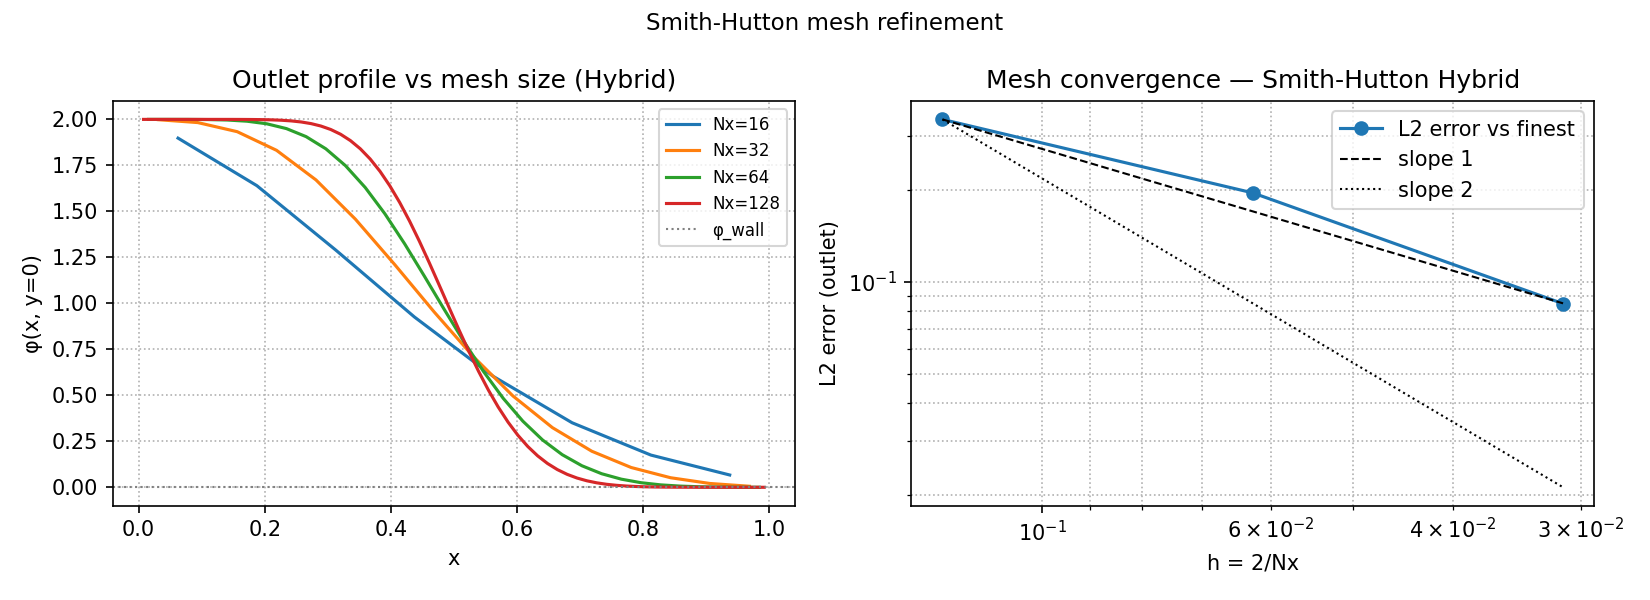
\includegraphics[width=\linewidth]{Chapter2/Media/SHRefine.png}
    \caption{Mesh refinement study for the Smith-Hutton case ($\rho/\Gamma = 10^3$, Hybrid). Left: exit profile $\phi(x, 0)$ for each mesh level. Right: $L_2$ error against mesh spacing $h = 2/N_x$; reference slope lines indicate first- and second-order convergence rates.}
    \label{figConvRefinement}
\end{figure}


\subsubsection{Model Validation}
The model is validated by running the Smith-Hutton problem for three convective schemes — CDS, UDS, and Hybrid — across all three values of $\rho/\Gamma$, using the mesh resolution established by the refinement study. The three schemes represent different points in the accuracy-stability trade-off described in Table~\ref{tabConvSchemes}: CDS is second-order accurate but loses diagonal dominance for $|Pe_k| > 2$, which causes oscillations; UDS maintains diagonal dominance at all Peclet numbers but is only first-order accurate; and the Hybrid scheme applies CDS where $|Pe_k| \leq 2$ and switches to UDS above that threshold. This range of behaviours is expected to produce clearly different exit profiles as $\rho/\Gamma$ increases and convection becomes dominant.

For each $\rho/\Gamma$ case, two quantities are reported: the number of inner solver iterations and the final residual, which assess convergence and stability; and the exit profile $\phi(x,\, y=0)$, which is compared directly against the reference values~\cite{SmithHutton1982}. The steady-state $\phi$ colormaps for all three schemes are also provided to give a visual assessment of the transport behaviour and to expose the CDS divergence at high Peclet numbers. The results are presented in Figs.~\ref{figConvNumerical},~\ref{figConvSH}, and~\ref{figConvUDS}.

\begin{figure}[ht]
    \centering
    \begin{tabular}{cc}
        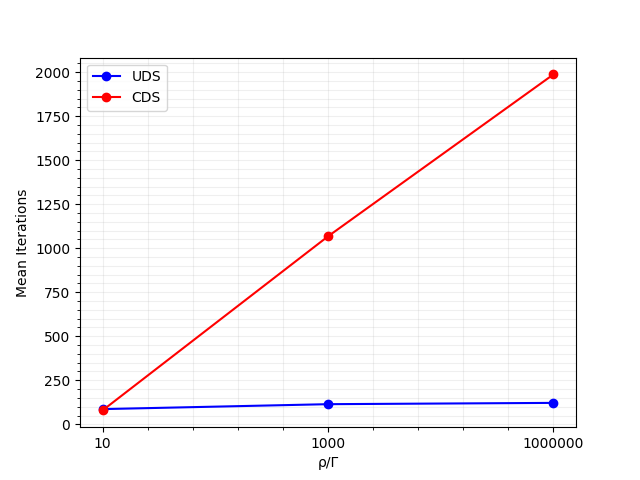
\includegraphics[width=0.45\linewidth]{Chapter2/Media/IterConv.png} & 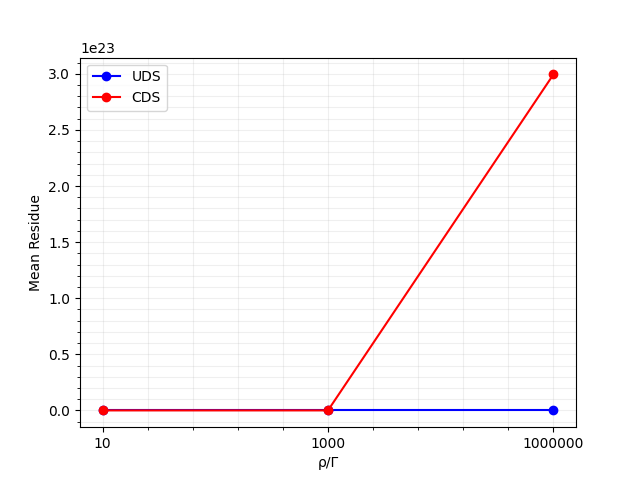
\includegraphics[width=0.45\linewidth]{Chapter2/Media/ResidueConv.png} \\
    \end{tabular}
    \caption{Number of iterations (left) and solver residual (right) for the three convective schemes across all $\rho/\Gamma$ cases.}
    \label{figConvNumerical}
\end{figure}

\begin{figure}[ht]
    \centering
    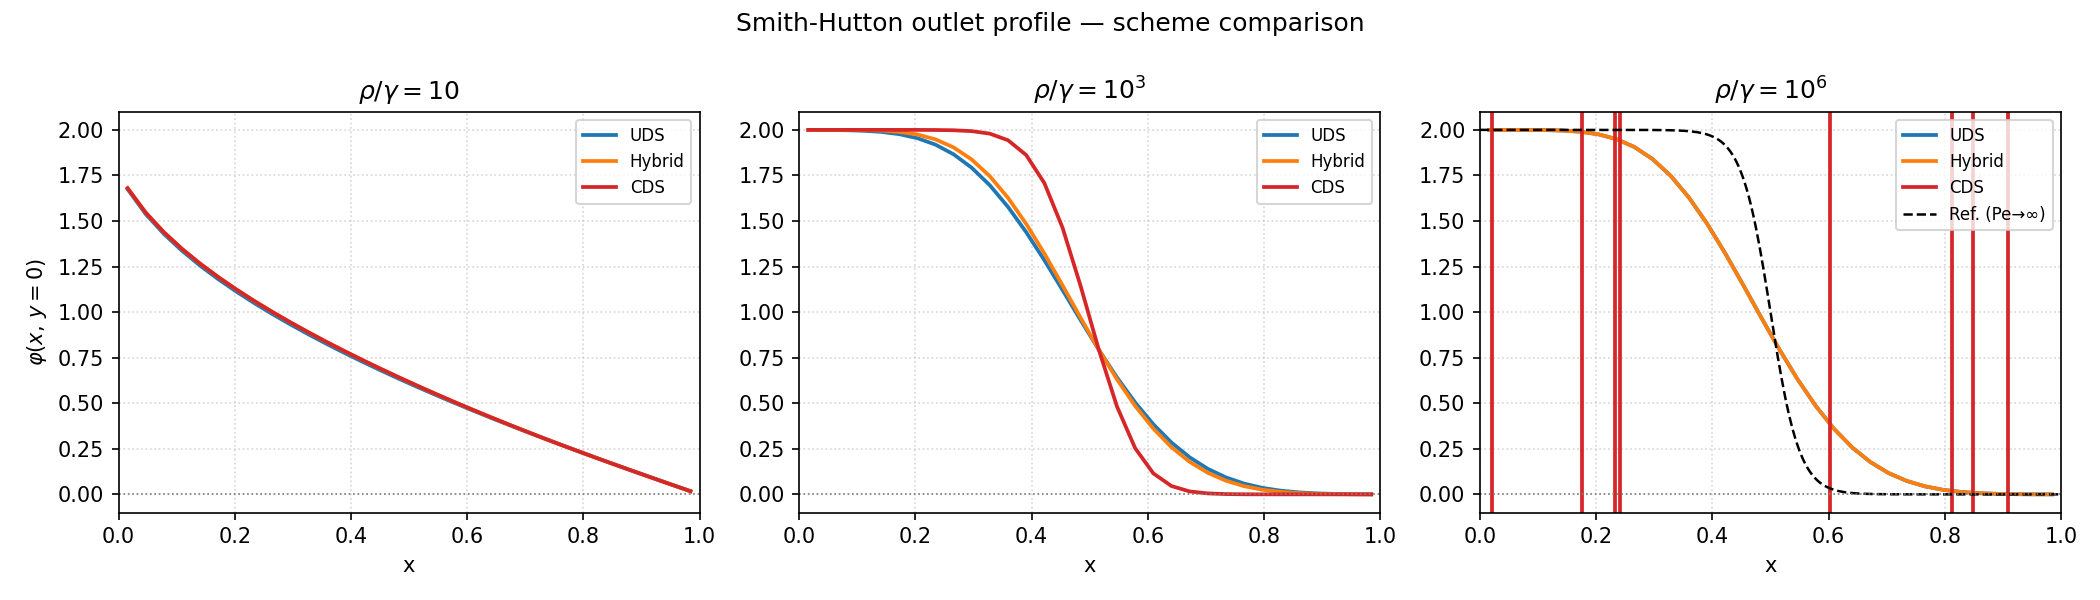
\includegraphics[width=\linewidth]{Chapter2/Media/SHSchemeComparison.png}
    \caption{Exit profile $\phi(x, 0)$ for CDS, UDS, and Hybrid compared against the reference of Smith and Hutton~\cite{SmithHutton1982} at each $\rho/\Gamma$ case. For $\rho/\Gamma = 10^6$ the reference corresponds to the $Pe \to \infty$ limit.}
    \label{figConvSH}
\end{figure}

\begin{figure}[ht]
    \centering
    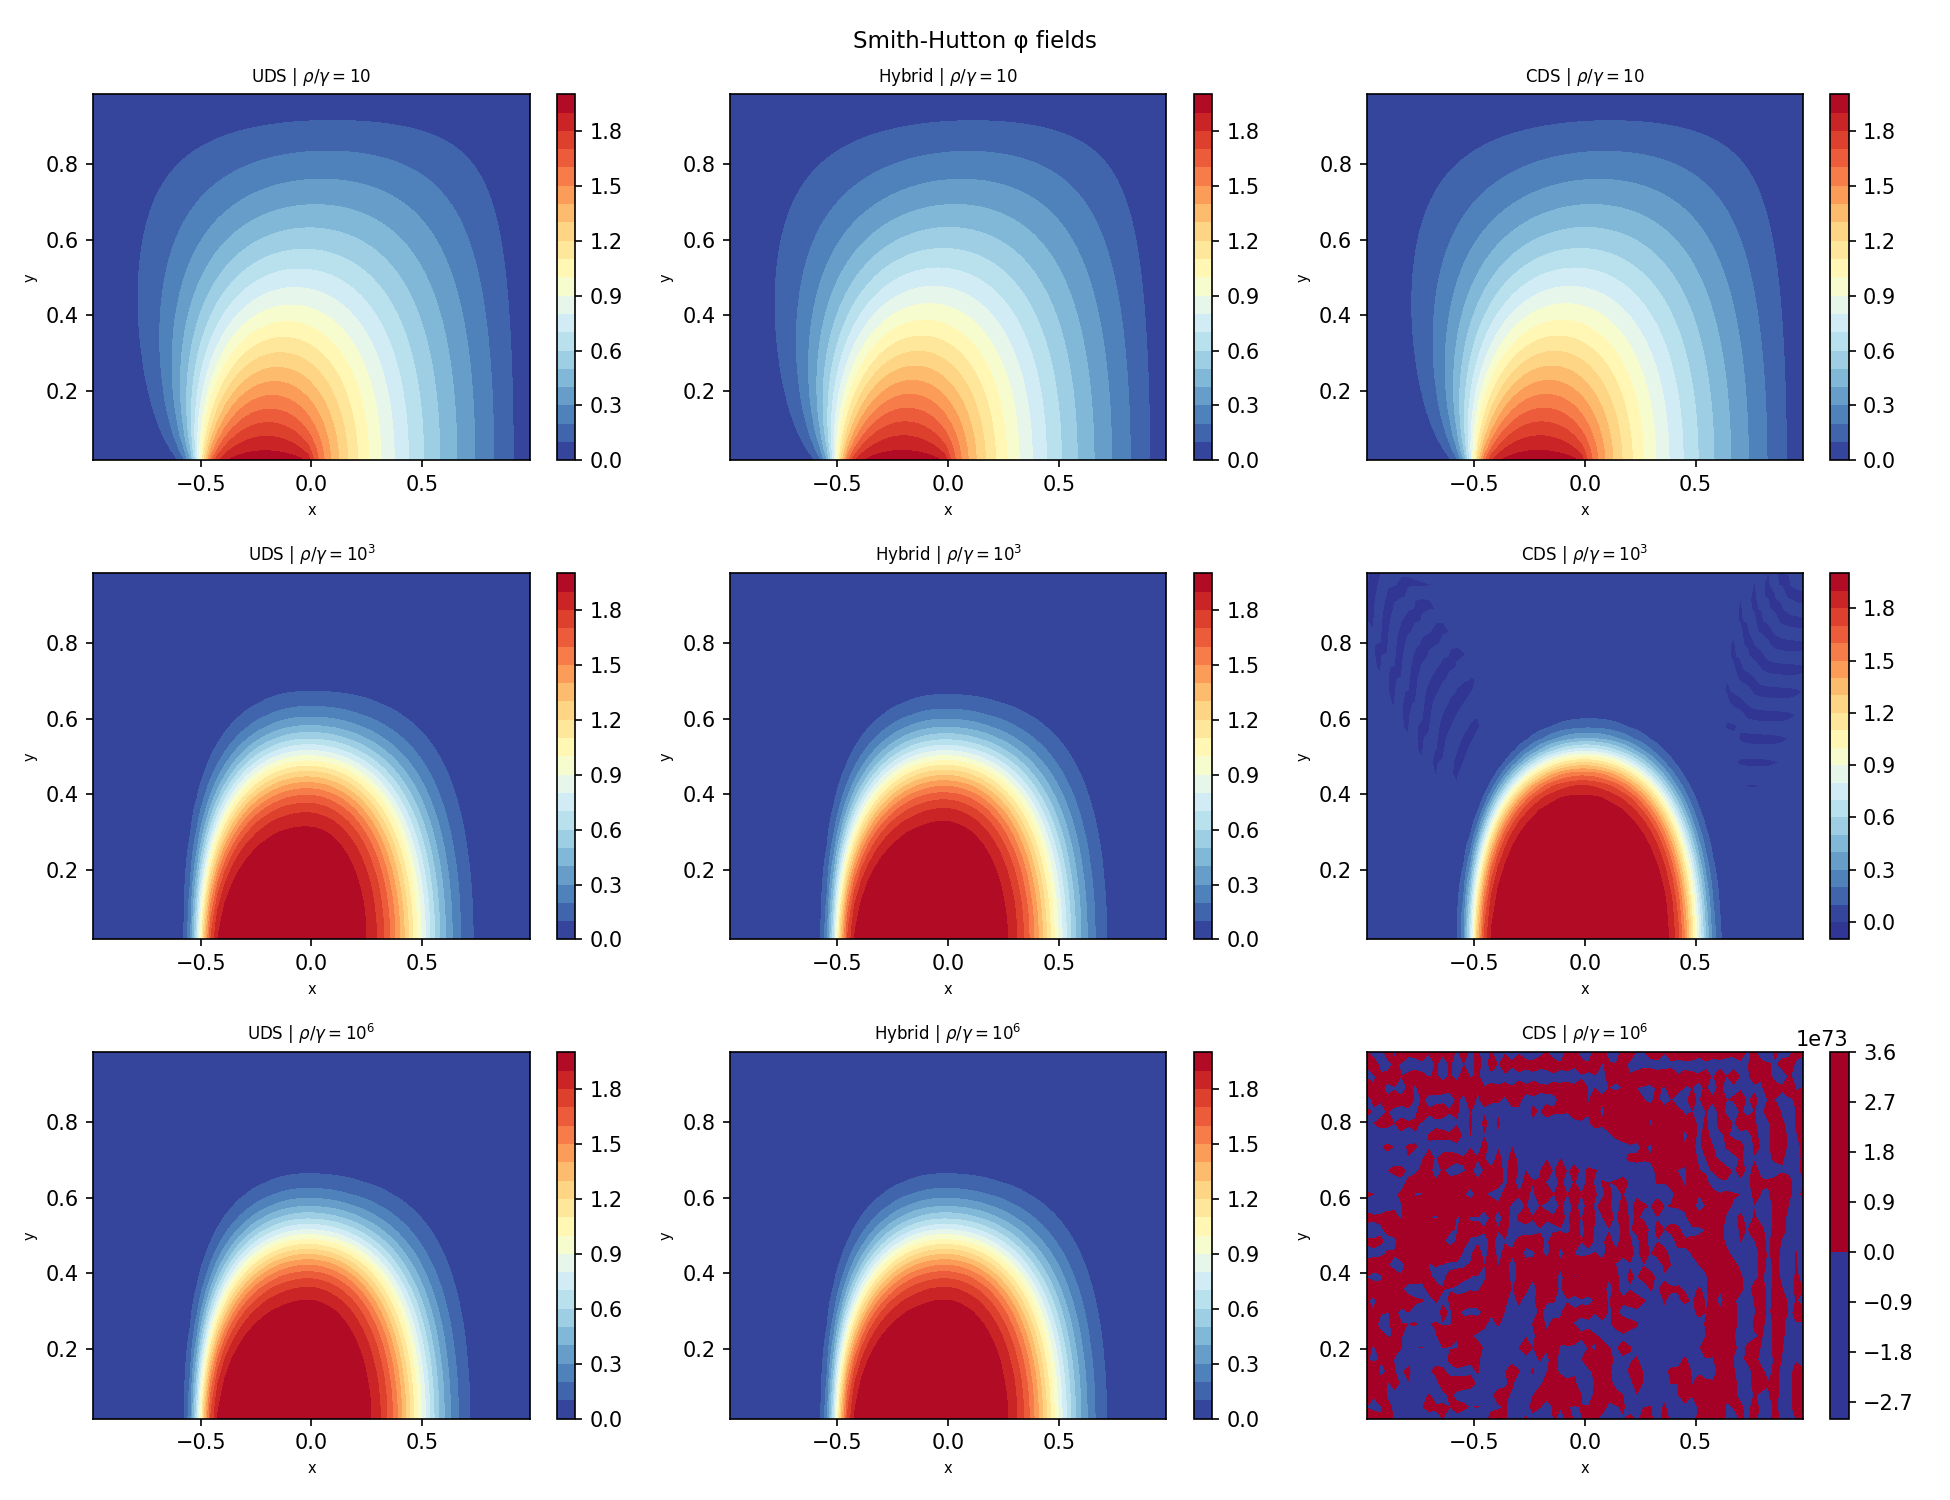
\includegraphics[width=\linewidth]{Chapter2/Media/SHSchemeFields.png}
    \caption{Steady-state $\phi$ field for UDS (left column), Hybrid (centre column), and CDS (right column) across all three $\rho/\Gamma$ cases (rows). At $\rho/\Gamma = 10^6$ the CDS solution has diverged and is shown at the scale of the numerical overflow.}
    \label{figConvUDS}
\end{figure}


\chapter{Convection-Diffusion Model}~\label{chapNavierStokes}

This chapter will describe the implementation of a numerical solver for the Navier-Stokes Equations. 




\section*{Conclusions}

These document has covered the development and evolution of a Heat and Mass Transfer solver across different benchmarks of increasing complexity. Across the different stages of development of this model, different complexities regarding the implementation of numerical methods and the simplification of physical models have been observed and analyzed. In addition, the model developed during this project will serve as a stepping stone towards more complex implementations. There are still several improvements that can be made to the model, particularly in terms of optimization of variables and standarization of certain algorithms. The model will continue to be maintained to expand its capacity and increase its performance.

\begin{enumerate}
    \item The Pure Diffusion Model served as a first step in defining the architecture of the model. This structure consists of the 5 main components (Material, Mesh, Discretizer, Solver, and Probe) that handle the different operations required for the solver; storing data about the domain, about the physical phenomena, solving the model, and storing the desired results. This system allows for organized and easy-to-read code, which makes it easier to work on long-term maintenance of the model. Furthermore, this model was used as a baseline comparison for the linear solvers implemented in the model (GS and CG).
    \item The Convection Diffusion Model served as an introduction to the advective scheme, which determines the numerical approach for approximating the convective effect of flow at the walls. The formulation proposed by Patankar allows for a standardized model that can handle different advective schemes under a single formulation. It is important to highlight the observed behaviour of CDS when used to solve convection-dominant problems, as this model can lose diagonal dominance for $|Pe| > 2$, showing a checkerboarding effect. For high $Pe$ cases on the other hand, UDS can provide a more stable solution while sacrificing precision due to gradient smoothing. 
    \item The Navier-Stokes Model introduced the Fractional Step Method, which consists of separating the velocity components from the pressure component and solving them discretely by using the Adams-Bashforth discretization method to obtain second order accuracy. Furthermore, Staggered Meshes were used to eliminate the need for interpolating values at the faces; choosing to locate them at the required locations from the start. Finally, the difference between a diffusion-dominant and convection-dominant scenario was also evident in this tests. However, since the velocity is decoupled and calculated explicitly with Adams-Bashforth, the same checkerboarding apparent for the convection-diffusion case was not seen here.
    \item All models were succesfully validated against the benchmark reference values. 
\end{enumerate}


\subsection{Future Work}

\begin{enumerate}
    \item During the development of the model, the code architecture has changed significantly. As the model kept expanding the, new variables and structs were introduced to store the required information and better organize the code. While there were several changes in structure when moving from a pure-diffusion model to a convection-diffusion model, the main changes (particularly to the Mesh) were made when moving to the Navier-Stokes model. Since the first two models solved a single transport variable, Mesh.cpp stored all relevant variables directly. On the other hand, the NS solver requires multiple transport variables to be evaluated at the same time; and as such, they require their own set of variables for that purpose. For this purpose, a cleaner struct implementation was developed that organizes each transport variable independently and stores different metadata to reduce the operations done by the discretizer. The convection-diffusion solver should be modified to operate under the same parameters, modifying the logic to fit the new struct definition and standardizing the model.
    \item The current model can still be expanded to support more complex cases, with the next step being solving natural convection problems. This requires the inclusion of the energy conservation equation in the model as well. In addition, the current model can still be extended to support a 3D domain; however, this change implies a larger overhaul of several functions in the model and will be considered for implementation at a later date.
    \item Further studies about the nature of the numerical solver can be included to deepen the understanding and implication of this decisions. For instance, only CDS and UDS were tested during the development of this project even thought the Hybrid, Exponential, and Power Law schemes are also implemented. With more time and computational resources, additional tests for the 5 different schemes could be done in different edge scenarios.
\end{enumerate}


% Bibliography
\clearpage
\phantomsection
\addcontentsline{toc}{section}{Bibliography}
\bibliographystyle{unsrt}
\bibliography{bibliography}



% HAVEN'T DONE THIS YET
% \appendix
% \include{app1/app1}

% \refstepcounter{chapter}
% \section*{Nomenclature}
\addcontentsline{toc}{section}{Nomenclature}

\subsection*{Roman Symbols}
\begin{tabular}{@{}lll@{}}
    $A$              & Coefficient matrix of the linear system              & [--] \\
    $a_P$            & Diagonal coefficient of the discretized equation     & [--] \\
    $a_k$            & Off-diagonal coefficient for neighbour $k$           & [--] \\
    $A(|Pe|)$        & Patankar's interpolation function                    & [--] \\
    $b_P$            & Right-hand side source term                          & [--] \\
    $c_p$            & Specific heat capacity                               & [J\,kg$^{-1}$K$^{-1}$] \\
    $D_k$            & Diffusive conductance at face $k$                    & [--] \\
    $e_N$            & $L_2$ error of the exit profile at mesh level $N$   & [--] \\
    $F_k$            & Convective mass flux at face $k$                    & [kg\,s$^{-1}$] \\
    $g$              & Gravitational acceleration                           & [m\,s$^{-2}$] \\
    $h$              & Convective heat transfer coefficient                  & [W\,m$^{-2}$K$^{-1}$] \\
    GCI              & Grid Convergence Index                               & [--] \\
    $H$              & Cavity height / domain characteristic length         & [m] \\
    $L$              & Domain length                                        & [m] \\
    $N$              & Number of nodes per side                             & [--] \\
    $\overline{Nu}$  & Average Nusselt number                               & [--] \\
    $Nu_\text{max}$  & Maximum local Nusselt number at the hot wall         & [--] \\
    $p$              & Apparent convergence order                           & [--] \\
    $P$              & Pressure                                             & [Pa] \\
    $Pe$             & Cell Péclet number                                   & [--] \\
    $Pr$             & Prandtl number ($\nu/\alpha$)                        & [--] \\
    $q_V$            & Volumetric heat generation rate                      & [W\,m$^{-3}$] \\
    $\dot{q}$        & Heat flux                                            & [W\,m$^{-2}$] \\
    $Ra$             & Rayleigh number                                      & [--] \\
    $Re$             & Reynolds number                                      & [--] \\
    $S_P$            & Source term per unit volume                          & [varies] \\
    $T$              & Temperature                                          & [K or \textdegree C] \\
    $t$              & Time                                                 & [s] \\
    $u$              & Horizontal ($x$-direction) velocity component        & [m\,s$^{-1}$] \\
    $U$              & Lid velocity (LDC benchmark)                         & [m\,s$^{-1}$] \\
    $u_\text{min}$   & Minimum $u$-velocity along the vertical centreline   & [m\,s$^{-1}$] \\
    $v$              & Vertical ($y$-direction) velocity component          & [m\,s$^{-1}$] \\
    $\mathbf{v}$     & Velocity vector                                      & [m\,s$^{-1}$] \\
    $V_P$            & Control volume                                       & [m$^3$] \\
    $x,\,y$          & Spatial coordinates                                  & [m] \\
\end{tabular}

\subsection*{Greek Symbols}
\begin{tabular}{@{}lll@{}}
    $\alpha$                  & Thermal diffusivity ($\lambda/\rho c_p$)         & [m$^2$\,s$^{-1}$] \\
    $\beta$                   & Thermal expansion coefficient                    & [K$^{-1}$] \\
    $\delta$                  & Hyperbolic tangent mesh clustering parameter     & [--] \\
    $\Delta t$                & Time step                                        & [s] \\
    $\Delta x,\,\Delta y$     & Cell width in $x$- and $y$-direction             & [m] \\
    $\varepsilon$             & Convergence tolerance                            & [--] \\
    $\varepsilon_\text{temporal}$ & Temporal steady-state tolerance             & [--] \\
    $\Gamma$                  & Diffusion coefficient                            & [kg\,m$^{-1}$s$^{-1}$] \\
    $\lambda$                 & Thermal conductivity                             & [W\,m$^{-1}$K$^{-1}$] \\
    $\mu$                     & Dynamic viscosity                                & [Pa\,s] \\
    $\nu$                     & Kinematic viscosity ($\mu/\rho$)                 & [m$^2$\,s$^{-1}$] \\
    $\rho$                    & Density                                          & [kg\,m$^{-3}$] \\
    $\phi$                    & General transported scalar variable              & [--] \\
    $\omega$                  & BiCGSTAB local-minimisation step length          & [--] \\
\end{tabular}

\subsection*{Subscripts and Superscripts}
\begin{tabular}{@{}ll@{}}
    $P,\,W,\,E,\,S,\,N$    & Cell centre node and its four cardinal neighbours \\
    $w,\,e,\,s,\,n$        & West, east, south, north cell faces \\
    $h,\,c$                & Hot wall, cold wall (DHC) \\
    $\text{ref}$           & Reference value \\
    $\infty$               & Far-field fluid value or Richardson-extrapolated limit \\
    $n,\,n+1$              & Current and next time level \\
    $k$                    & Face index \\
\end{tabular}

\subsection*{Abbreviations}
\begin{tabular}{@{}ll@{}}
    BC       & Boundary Condition \\
    BiCGSTAB & Bi-Conjugate Gradient Stabilized (linear solver) \\
    CDS      & Central Difference Scheme \\
    CFD      & Computational Fluid Dynamics \\
    CG       & Conjugate Gradient (linear solver) \\
    DHC      & Differentially Heated Cavity \\
    FSM      & Fractional Step Method \\
    FVM      & Finite Volume Method \\
    GCI      & Grid Convergence Index \\
    GS       & Gauss-Seidel (linear solver) \\
    HT       & Heat Transfer \\
    LDC      & Lid-Driven Cavity \\
    NS       & Navier-Stokes \\
    SH       & Smith-Hutton \\
    SPD      & Symmetric Positive Definite \\
    UDS      & Upwind Difference Scheme \\
\end{tabular}



\end{document}
